%%%%%%%%%%%%%%%%%%%%%%%%%%%%%%%%%%%%%%%%%%%%%%%%%%%%%%%%%%%%
%%% PRX Life submission --- A theory of templating substrates
%%% v15 --- adds Discussion scoping paragraph positioning the
%%%        framework against orthogonal preconditions of
%%%        life-as-we-know-it (metabolism, compartmentalization,
%%%        sustained chemical driving). Placed as penultimate
%%%        Discussion paragraph for reviewer skim-visibility
%%%        (reviewers read abstract / end-of-paper / methods first).
%%%        All formal content unchanged from v14.
%%% Compile with pdflatex; bibliography handled by bibtex (apsrev4-2.bst)
%%% Requires REVTeX 4.2 (texlive-publishers); APS submission portal compiles natively.
%%%%%%%%%%%%%%%%%%%%%%%%%%%%%%%%%%%%%%%%%%%%%%%%%%%%%%%%%%%%

\documentclass[aps,prx,reprint,amsmath,amssymb,floatfix,superscriptaddress,nofootinbib]{revtex4-2}

\usepackage{amsthm}
\usepackage{graphicx}
\usepackage{subcaption}
\usepackage{hyperref}
\usepackage{booktabs}
\usepackage{xcolor}

% Figure path: update to match the directory holding the current figure
% files. Bump in lockstep with manuscript version when figures are
% regenerated.
\graphicspath{{paper/figures/v15/}}

% subcaption configured so panel labels render as bold uppercase A, B, C, ...
\renewcommand{\thesubfigure}{\Alph{subfigure}}
\captionsetup[subfigure]{labelformat=simple,labelsep=space,font=bf,singlelinecheck=false}

% Zenodo DOI for the deposited code/data/dispatches archive (v0.0-prereg release).
\newcommand{\zenodoDOI}{\href{https://doi.org/10.5281/zenodo.20060972}{10.5281/zenodo.20060972}}

% Theorem environments — REVTeX doesn't predefine these
\newtheoremstyle{plain-thm}
  {3pt}{3pt}{\itshape}{}{\bfseries}{.}{ }{}
\theoremstyle{plain-thm}
\newtheorem{theorem}{Theorem}
\newtheorem{proposition}[theorem]{Proposition}
\newtheorem{corollary}[theorem]{Corollary}

\newtheoremstyle{definition-thm}
  {3pt}{3pt}{}{}{\bfseries}{.}{ }{}
\theoremstyle{definition-thm}
\newtheorem{definition}[theorem]{Definition}
\newtheorem{remark}[theorem]{Remark}

% Custom command for inline framework notation
\newcommand{\Istructpop}{I_{\mathrm{struct}}^{\mathrm{pop}}}
\newcommand{\Istructchan}{I_{\mathrm{struct}}^{\mathrm{chan}}}
\newcommand{\fphase}{f_{\mathrm{phase}}}
\newcommand{\fmonomer}{f_{\mathrm{monomer}}}
\newcommand{\Csub}{C_{\mathcal{S}}}
\newcommand{\Hbin}{h_b}
\newcommand{\descX}{\varphi_X}
\newcommand{\descY}{\varphi_Y}
\newcommand{\KL}[2]{D_{\mathrm{KL}}\!\left(#1 \,\|\, #2\right)}
\newcommand{\Xset}{\mathcal{X}}
\newcommand{\Sset}{\mathcal{S}}
\newcommand{\Op}{\mathcal{O}}
\newcommand{\liminff}{\liminf_{L\to\infty}}
\newcommand{\Reach}{\mathcal{R}}

\begin{document}

\title{A substrate recursion principle for biological information, with empirical anchoring through a templating-mode taxonomy}

\author{Sreedhar Volet}
\affiliation{Indras Bioinformatics, Hyderabad, India}

\author{Boggavarapu Kiran}
\affiliation{Department of Chemistry and Physics, McNeese State University, Lake Charles, LA 70609, USA}
\email{kiran@mcneese.edu}

\date{\today}

\begin{abstract}
Biological inheritance can be treated as a class of catalytic templating reactions in which a daughter molecule, generated by a kinetic kernel acting on a parent template, is itself a substrate for the next round of the same catalysis. We give the physicochemical conditions under which such a reaction can support unbounded heritable molecular distinguishability. Four conditions on the template--operator pair --- nonzero per-site information content under the active-site recognition kernel (R1), a count of independently variable recognized positions that grows without bound as the reaction extends (R2), catalytic closure under iteration possibly through a reversible involution such as Watson--Crick complementation (R3), and stochastic drift of the kernel in its recognition alphabet (R4) --- together with a scope condition (R5: the kernel is intrinsic physicochemistry, not externally optimized search), organize the analysis. We separate two necessity results that the prior literature conflated. The \emph{capacity theorem} states that linear scaling of substrate Shannon capacity with reaction extent requires R1, R2, R3 but not R4: a perfect copier transmits an exponentially large configurational ensemble while producing no novelty. The \emph{generation theorem} states that diversification of the heritable configuration set beyond the deterministic closure of a finite initial repertoire requires R4 in addition: branching trajectories in the recognized alphabet are needed for innovation. Population-level kinetics follow as a corollary (bounded heredity, organizing six attested templating reactions into a taxonomy) and a finite-population, finite-horizon proposition (tested over five inheritance kinetic schemes M0--M4; only individual-level stochastic drift reaches the target in the model class). A descriptor-relative diagnostic apparatus operationalizes the framework on the Drt3 reverse-transcriptase system: Drt3b is identified as a Mode~3 cyclic-conformational templating channel; the E26Q active-site mutant matches the analytic prediction for marginal G fraction ($0.10$; observed $0.1016$); AbiK same-fold non-templating is excluded; family-level analysis across 1{,}232 homologs is consistent with Mode~3 across the family and predicts a 15.7-fold dG elevation in 6 E26$\to$D primary-gate clades. Substitutions at two universal gate residues --- R253 (architectural) and G248 (selectivity) --- give single-experiment site-directed-mutagenesis falsification targets.
\end{abstract}

\maketitle

\section*{Popular Summary}

A bacterial defense protein called Drt3b, recently characterized in \emph{E. coli}, synthesizes DNA with a strict alternating ACAC pattern without copying any template. Two conserved active-site residues, Glu26 and Arg253, are modeled as enforcing an alternating two-state catalytic cycle that selects which nucleotide enters at each step. This is sequence without a sequence template, and it does not fit the textbook picture of inheritance.

We treat inheritance as a class of catalytic templating reactions and ask which chemistries can support open-ended evolution. We separate two requirements that have been conflated. \emph{Capacity} --- the ability to transmit exponentially many distinct heritable configurations --- requires three conditions on the template--catalyst pair: more than one monomer state recognized at each position, a position count that grows unboundedly with the reaction extent, and applicability of the catalysis to its own product. \emph{Generation} of novel heritable configurations beyond what is already present requires a fourth condition: stochastic drift of the catalysis in its recognition alphabet. A perfect copier has capacity but cannot innovate; a drifting copier has both. Drt3b fails the second capacity condition: its cycle has two states regardless of product length. The framework classifies six attested biological templating reactions as instances or partial instances of the same chemical specification and identifies two single-residue substitutions at Drt3b's active site whose effects would falsify the framework if measured.


\section{Introduction}

Biology runs on a small number of chemically distinct templating reactions for transmitting information across generations. DNA replication and ribosomal translation are the textbook cases: processive, ATP/GTP-coupled, polymerase- and ribosome-catalyzed monomer-by-monomer synthesis on a directing template. Prion propagation and amyloid templating add a second class --- a conformational attractor propagated across protein molecules through nucleation-and-elongation chemistry \citep{Greenwald2016}. Modular biosynthetic assemblies (non-ribosomal peptide synthetases, polyketide synthases) compose a third: a spatial sequence of catalytic modules executes a fixed sequence of condensation reactions, with the product specified by the active-site chemistry of each module \citep{Walsh2001}. The eukaryotic ciliate cortex constitutes a fourth: cortical patterns of basal-body orientation are inherited at division through the action of the existing cortical lattice on newly assembled units, with grafted inverted patches propagating as inverted for hundreds of cell generations without genomic change \citep{BeissonSonneborn1965, Frankel1989}. The recent characterization of bacterial defense-related templating systems --- the DRT family \citep{Deng2026, DRT1preprint2026, DRT7preprint2026} --- adds at least one more: Drt3b synthesizes alternating poly(AC) DNA without using a nucleic acid template, generating its product through a cyclic active-site catalytic mechanism rather than through Watson-Crick complementarity to an existing strand \citep{Deng2026}.

These reactions pose a physicochemical question, not a purely biological one: what conditions on a template--catalyst pair are necessary for it to support unbounded heritable molecular distinguishability under repeated catalytic action? The mechanisms have unrelated active-site chemistries, but their dynamical signatures separate cleanly. DNA replication transmits a configurational ensemble whose Shannon capacity grows linearly with sequence length. Prion propagation transmits a finite conformational free-energy minimum and accumulates nothing comparable. The field has no quantitative chemical-physics account of which reactions sit on which side of this line. What does a template--catalyst pair need to be for the configurational ensemble it transmits to grow unboundedly with reaction extent? Which catalytic chemistries qualify, which do not, and on what physicochemical basis is the line drawn? These questions are surprisingly absent from the current literature, despite half a century of attempts to address adjacent ones.

The attempts have approached the substrate-level question from three directions. The information-theoretic line --- \citet{Eigen1971}, \citet{EigenMcCaskillSchuster1989}, and \citet{Szathmary2000} --- treats copying-with-variation as a process whose stability depends on per-site error rate relative to genome length, generating the quasispecies framework and the error threshold $\mu^* \approx \log \sigma / L$. This work tells us how a substrate-borne replication process can fail dynamically (above threshold, the master sequence is lost) but not what makes a physical system a substrate at all. \citet{Szathmary2000} introduced the distinction between limited and unlimited heredity --- a substrate with $K$ possible states transmits limited heredity ($\log_2 K$ bits ceiling), while sequence-based substrates transmit unlimited heredity ($L \log_2 |\mathcal{A}|$, scaling with length). The distinction is intuitive and correct in spirit, but it is not formalized as a structural condition on substrates; it is asserted as a typological observation.

A second line --- \citet{Hull1980}, \citet{MaynardSmith2000} --- specifies abstract requirements on a replicator (faithful self-copying, heritable variation in fitness) without committing to any particular chemistry that realizes those requirements. This work supplies criteria a unit of selection must meet but is chemistry-blind: it does not specify which physical realizations of the abstract requirements actually occur, and through what catalytic mechanism.

The substrate-level line --- \citet{Schrodinger1944}'s aperiodic crystal, the GARD-class compositional inheritance models \citep{Kauffman1986, Hordijk2012}, and \citet{Pross2011}'s dynamic kinetic stability --- has attempted to specify the physical substrate directly. Schr\"odinger's gestural answer (the chromosome is an aperiodic crystal whose information is in its sequence of distinct molecular groups) was prescient but not formalized. GARD-class models attempted a formal substrate-level alternative: a compositional set of catalytic molecules can transmit information across generations through preferential reproduction of similar compositions. \citet{Vasas2010} showed using GARD's own machinery that compositional inheritance fails the fidelity requirements for open-ended evolution: high-fidelity compositional transmission requires a lognormal distribution of catalytic rate constants so narrow as to be biologically unrealistic. The result is a clear empirical verdict (compositional inheritance does not work), but it does not generalize: it tells us GARD fails, not what any substrate must satisfy to succeed.

What is missing from all three lines is a single statement, at the chemical-physics level of the template--catalyst pair, of what conditions are necessary for a templating reaction to transmit unbounded heritable distinguishability. The information-theoretic work treats population dynamics on a given templating reaction, not the reaction itself. The replicator-criteria work is chemistry-blind. The substrate-level work has either gestured (Schr\"odinger) or been falsified (GARD). The Drt3b finding sharpens the gap: Drt3b is unambiguously biological, unambiguously templating, and unambiguously not a sequence-template polymerase. A framework that classifies it has to be at the level of the catalytic mechanism itself.

We give such a framework here. Four conditions on the template--catalyst pair --- nonzero per-site information content under the active-site recognition kernel (R1), a count of independently variable recognized positions that grows without bound with the reaction extent (R2), catalytic closure under iteration, possibly through a reversible involution such as Watson--Crick complementation (R3), and stochastic drift of the kernel in its recognition alphabet (R4) --- together with a scope condition (R5: the kernel is intrinsic physicochemistry rather than externally optimized search), organize the analysis. We separate two necessity results that earlier formulations of this work conflated --- a capacity theorem (R1, R2, R3 necessary for linear scaling of substrate Shannon capacity) and a generation theorem (R4 additionally necessary for diversification of the heritable configuration set beyond the deterministic closure of a finite initial repertoire). Capacity is storage architecture under the catalytic kernel; generation is stochastic branching to neighboring configurations under the same kernel; both are needed for biology's open-ended evolution, and they have different chemical requirements. The Results that follow present the formal statements, a bounded-heredity corollary that organizes six attested templating reactions into a taxonomy, a finite-population proposition tested over five inheritance kinetic schemes (M0--M4), and a descriptor-relative diagnostic apparatus that operationalizes the framework on the Drt3 reverse-transcriptase system with quantitative match to the published biochemistry and two single-experiment site-directed-mutagenesis falsification targets at universal-gate residues.

A note on vocabulary. We use ``drift'' rather than ``error'' or ``variation'' for the stochastic part of the catalytic kernel: the kernel produces what its physics produces, and there is no externally imposed target configuration the catalysis is trying to reach. We retain ``error'' for established field usage (Eigen's threshold, per-position misincorporation rate $\varepsilon$ against a defined Watson--Crick canonical product), where the technical meaning is fixed.

Population-genetic theory describes which gene variants persist under selection but takes the inheritance reaction itself as given. We treat the reaction itself. The result, developed below, is that biology's open-ended evolution is hosted not by ``copying with variation'' in the abstract but by a specific class of templating chemistries: those whose active-site recognition kernel resolves multiple monomer species per position (R1), whose product length carries independently variable recognized positions extensively in the reaction extent (R2), whose product is itself a substrate for the same kernel (R3), and whose kernel is genuinely stochastic in its recognition alphabet (R4). Capacity and generation are separable structural requirements within this class.


\section{Results}

\subsection{The substrate recursion principle: structural conditions and necessity}

We state the principle in three parts: definitions of heredity capacity and cumulative generation, the substrate recursion conditions, and two necessity theorems separating capacity from generation. We give each formal statement after a brief plain-language framing of what it claims, and follow each with a biological example showing what the formalism captures.

\paragraph{Definition 1: heredity capacity and cumulative generation.}

Before specifying conditions on the substrate, we have to specify what the substrate is required to support. ``Open-ended information generation'' has been used loosely in the literature, and the looseness has hidden a quantifier ambiguity that determines which structural conditions are necessary. We separate two formal notions.

The first is \emph{substrate heredity capacity}: how much information the substrate can transmit per recursion event, treated as an encoder property. The substrate's capacity is the supremum of mutual information across all admissible input distributions:
\begin{equation}
\Csub(L) = \sup_{\Pi_X} I\!\left(\descX(X);\, \descX(X')\right), \quad X' \sim Q_L(\cdot \mid X).
\label{eq:capacity}
\end{equation}
The substrate has \emph{unlimited heredity capacity} if $\Csub(L) = \Omega(L)$; equivalently, in the discrete noiseless limit, if the set of heritably distinguishable and recursively readable configurations $\Reach_L$ satisfies $|\Reach_L| \ge 2^{cL}$ for some $c > 0$. Capacity is a property of the substrate-operation pair under \emph{any} input ensemble; it includes the case where many initial configurations exist simultaneously.

The second is \emph{cumulative generative recursion}: the substrate's ability, starting from a finite initial repertoire $S_0 \subsetneq \Xset_L$ that is small compared to the substrate's reachable set, to produce heritable configurations \emph{beyond the deterministic closure of $S_0$ under $\Op$}, through branching local alternatives in the same recognized alphabet. The qualifier ``beyond the deterministic closure'' is essential: a deterministic operation can leave $S_0$ (e.g., a counter chain $000 \to 001 \to 010 \to \cdots$ generates configurations outside any singleton $S_0$), but the descendant set is then a single predetermined orbit. Cumulative generation in the chemical-kinetics sense requires that the future is not pre-specified --- that the kernel produces heritable branching alternatives in $\Sigma$ at each step, so the descendant set is genuinely larger than the deterministic orbit closure.

Formally, let $\mathrm{cl}_{\det}(S_0)$ denote the closure of $S_0$ under any deterministic restriction of $Q_L$ (taking, at each step from any $X$, a single fixed successor permitted by $Q_L$'s support). Then $(\Xset, \Op)$ supports cumulative generation if the recursively readable descendant set reachable from $S_0$ with positive probability under $Q_L$ strictly contains $\mathrm{cl}_{\det}(S_0)$ for all proper $S_0 \subsetneq \Xset_L$ with $|S_0| \ll |\Reach_L|$, with the additional configurations differing from elements of $\mathrm{cl}_{\det}(S_0)$ in local recognized-state positions (i.e., in the alphabet $\Sigma$).

\begin{definition}[Heredity capacity]
\label{def:capacity}
A substrate-operation pair $(\Xset, \Op)$ has \textnormal{unlimited heredity capacity} if $\Csub(L) = \Omega(L)$ as $L \to \infty$. Equivalently, in the discrete noiseless limit, $|\Reach_L| \ge 2^{cL}$ for some $c > 0$.
\end{definition}

\begin{remark}
The two formulations are coordinated through entropy: linear scaling of mutual information capacity ($\Csub(L) = \Omega(L)$ bits) is equivalent to exponential scaling of the recursively readable state count ($|\Reach_L| = \Omega(2^{cL})$). The first is the information-theoretic statement; the second is the combinatorial statement. They are not in conflict; they are the same fact at two levels of description.
\end{remark}

\begin{definition}[Cumulative generative recursion]
\label{def:generation}
A substrate-operation pair $(\Xset, \Op)$ supports \textnormal{cumulative generative recursion} if, for arbitrarily large $L$ and any proper finite initial repertoire $S_0 \subsetneq \Xset_L$ with $|S_0| \ll |\Reach_L|$, repeated application of $Q_L$ generates a recursively readable descendant set whose heritable descriptor support strictly contains the deterministic closure $\mathrm{cl}_{\det}(S_0)$, with the additional configurations arising through branching local alternatives in the same recognized alphabet $\Sigma$ as in (R1).
\end{definition}

DNA illustrates both. The $4^L$-configuration space gives unlimited heredity capacity; the polymerase's drift in the nucleotide alphabet gives cumulative generation. The two are conceptually independent: a hypothetical perfect copier of DNA satisfies Definition~\ref{def:capacity} (any of $4^L$ templates is faithfully preserved across iterations) but not Definition~\ref{def:generation} (the descendant set from a finite $S_0$ is exactly $\mathrm{cl}_{\det}(S_0) = S_0$ itself, with no branching alternatives in $\Sigma$). A purely deterministic-counter substrate (a hypothetical $000 \to 001 \to 010 \to \cdots$ chain) likewise fails Definition~\ref{def:generation}: the descendant set is bounded by the single deterministic orbit and the substrate does not produce heritable branching alternatives. Drt3b fails Definition~\ref{def:capacity} at the substrate level: at any product length, Drt3b's two-phase cyclic dynamics distinguish only $\log_2 2 = 1$ bit of phase, so $\Csub(L) = O(1)$.

A note on what the kernel does and does not encode. $Q_L(X' \mid X)$ is the distribution over outcomes that the active-site free-energy landscape, the available reactants, and the chemical driving (NTP hydrolysis or analogous energy source) produce when the catalysis acts on $X$. The kernel does not encode a target product; consequently, every template in iterated $Q_L$-application is the drifted product of prior runs of the same reaction, and no configuration is canonical at the kernel level. ``Drift'' rather than ``error'' is the appropriate vocabulary for the dispersion of $Q_L(X' \mid X)$ around any nominal consensus.

\paragraph{Definition 2: structural conditions on the substrate-operation pair.}

The substrate-operation pair $(\Xset, \Op)$ is the formal object the principle constrains. $\Xset_L$ is the space of admissible configurations of size $L$; $\descX(X) \in \Sigma^L$ is the descriptor of $X$ over the recognition alphabet $\Sigma$; $\Op$ is the operation with kernel $Q_L(X' \mid X)$ producing $X' = \Op(X)$, possibly composed with a reversible involution $\iota: \Xset_L \to \Xset_L$. The reversible involution covers the canonical case where the immediate product of $\Op$ is the complement of the input (Watson-Crick complementarity in DNA replication produces $\bar{X}$, and the next round of replication on $\bar{X}$ recovers $X$); the involution permits the recursion to close even when each individual $\Op$ application produces a complement rather than a copy.

Five conditions follow. Four are structural and are what the necessity theorem will require; the fifth is scope-defining and demarcates the domain to which the principle applies. We state them formally first, then walk through each in biological terms.

\begin{definition}[Substrate recursion conditions]
\label{def:conditions}
The substrate-operation pair $(\Xset, \Op)$ satisfies the substrate recursion conditions if:

\begin{description}
\item[(R1) Positive entropy per recognized site.] At each addressable position $i$, the recognition step in $\Op$ distinguishes at least two alternative monomer states drawn from a recognition alphabet $\Sigma$ with $|\Sigma| \ge 2$. The per-site entropy under the maximum-entropy distribution on the alphabet, $h_{\mathrm{site}} = \log_2 |\Sigma|$, is positive: $h_{\mathrm{site}} > 0$.

\item[(R2) Unbounded independently variable position count.] The substrate has non-recurrent sites whose count $N(L)$ grows unboundedly: $\liminf_{L \to \infty} N(L) = \infty$. ``Independently variable'' is meant in the first-order, descriptor-relative sense: increasing $L$ increases the count of heritable recognized degrees of freedom under the operation-relevant descriptor, and the substrate is \emph{not constrained to a finite recurrent phase repertoire}. The condition does not require that recognized states at distinct positions be statistically independent in any strong joint-distribution sense --- DNA polymerases exhibit context-dependent error rates and base composition biases, and DNA still satisfies R2 because the count of independently variable positions grows with sequence length. Composition vectors, homogeneous concentrations, and bulk mixtures fail R2 because they lack addressable position. Cyclic systems with finite recurrent phase repertoires fail R2 because $N(L)$ is bounded at the cycle length: product length can grow without bound while the count of heritable degrees of freedom remains at the cycle complexity $N$. This sharpening is what protects the Drt3b argument from a naive ``product length grows'' reading.

\item[(R3) Same-operation recursion (with allowed involution).] The output $X' = \Op(X)$ is structurally an element of $\Xset_L$ for which $\Op(X')$ is well-defined, possibly via a reversible involution $\iota$ such that $\Op(\iota(X')) \in \Xset_L$. The recursion takes the form
\[
X \xrightarrow{\Op} X' \xrightarrow{\Op} X'' \xrightarrow{\Op} \cdots \quad \text{or} \quad X \xrightarrow{\Op} \iota(X') \xrightarrow{\Op} X'' \xrightarrow{\Op} \cdots
\]
The condition excludes operations whose products are not readable by the same operation.

\item[(R4) Heritable local drift in the recognized alphabet.] The kernel $Q_L(X' \mid X)$ has nonzero probability of producing configurations $X' \neq X_{\mathrm{ref}}(X)$ for any reference configuration, with the drift lying in the same alphabet $\Sigma$ as the recognition step in (R1). Substrate content (the descriptor $\descX(X)$) and substrate templating function (the role of $X$ in $\Op(X) \to X'$) are the same physical entity: drift in content is drift in the next iteration's template. We use \emph{drift} rather than \emph{error} or \emph{variation}: the kernel produces what its physics produces, and the dispersion is a property of the kernel ensemble, not a departure from an external target.

\item[(R5) Scope: non-teleological intrinsic operation.] The kernel $Q_L$ depends only on the physicochemistry of $(\Xset, \Op)$, not on an externally specified target configuration, loss function, or convergence criterion. (R5) is scope-defining rather than structural: it demarcates the domain in which the structural conditions (R1)--(R4) apply. Differential persistence of configurations may occur downstream as a consequence of $\Op$'s action over a finite population, but selection acts on products, not on the operation itself. Systems whose operation is externally optimized (gradient descent on a loss function, designed catalytic cycles with specified targets) are outside the principle's scope.
\end{description}
\end{definition}

The conditions in biological terms:

\begin{itemize}
\item \textbf{(R1)} requires that the substrate's recognition step distinguishes at least two states at each site. DNA satisfies this: at each position, the polymerase distinguishes A, T, G, and C, giving $h_{\mathrm{site}} = 2$ bits. A system that recognizes only one state at each position --- a polymerase that incorporates only T --- has $h_{\mathrm{site}} = 0$ and fails (R1) at the recognition level.
\item \textbf{(R2)} requires that the count of independently variable sites grows without bound. DNA satisfies this: the polymer can extend arbitrarily, and increasing length increases the number of heritable recognized degrees of freedom, even though local sequence context can affect copying probabilities. Drt3b's cycle has only two phases regardless of product length; site count is bounded at 2, and (R2) fails.
\item \textbf{(R3)} requires that the substrate's operation can be applied to its own output. DNA replication satisfies this through the involution $X \to \bar{X}$: the daughter strand is itself a DNA strand, and a polymerase can replicate it. Ribosomal translation fails (R3): the protein product of translation is not a substrate the ribosome can re-read; recursion is recovered only through Mode 1 acting on the gene that encodes the ribosomal machinery.
\item \textbf{(R4)} requires that the substrate's operation produces drift, and that the drift lies in the alphabet the operation recognizes. DNA polymerases produce drift in the nucleotide alphabet (a $\sim 10^{-9}$ per-position rate against the Watson-Crick canonical product), and the drifted product is itself recognized at the next iteration. A perfect copier (zero drift) fails (R4); a system that produces drift in a different alphabet (chemical modifications that the polymerase does not read) also fails (R4).
\item \textbf{(R5)} requires that the operation is intrinsic physicochemistry, not externally specified. DNA replication satisfies this: the polymerase's catalytic action is not driven by an external loss function. A neural network trained by gradient descent toward a target distribution does not satisfy (R5): the operation is externally specified by the loss function and is therefore outside the principle's scope. (R5) does not say the externally optimized system fails biology; it says the principle's structural analysis does not apply to it.
\end{itemize}

\paragraph{Theorems 1 and 2: capacity and generation as separate necessity claims.}

The two definitions above let us state two distinct necessity claims that earlier formulations conflated. The first concerns heredity capacity (the substrate's encoder properties as an information channel); the second concerns cumulative generation (the substrate's ability to innovate from a finite seed). Both are necessary for the open-ended evolution biology exhibits, but they have different structural requirements, and the empirical phenomena are clearer when the two are separated.

\begin{theorem}[Capacity: necessity of R1, R2, R3 for unlimited heredity capacity]
\label{thm:capacity}
Within the scope defined by \textnormal{(R5)}, if a substrate-operation pair $(\Xset, \Op)$ has unlimited heredity capacity in the sense of Definition~\ref{def:capacity}, then it satisfies \textnormal{(R1)}, \textnormal{(R2)}, and \textnormal{(R3)}.
\end{theorem}

\begin{theorem}[Generation: necessity of R4 for cumulative generative recursion]
\label{thm:generation}
Within the scope defined by \textnormal{(R5)}, if a substrate-operation pair $(\Xset, \Op)$ supports cumulative generative recursion in the sense of Definition~\ref{def:generation} --- i.e., its descendant set from finite $S_0$ strictly contains $\mathrm{cl}_{\det}(S_0)$ through branching local alternatives in $\Sigma$ --- then it satisfies \textnormal{(R4)} in addition to \textnormal{(R1)}, \textnormal{(R2)}, and \textnormal{(R3)}.
\end{theorem}

\paragraph{Proof of Theorem~\ref{thm:capacity} (sketch).} The argument proceeds by upper-bound contrapositive. For any substrate-operation pair, the heredity capacity is bounded above by
\begin{equation}
\Csub(L) \le N(L) \cdot \log_2 |\Sigma|.
\label{eq:capacity_upper_bound}
\end{equation}
This holds because $\Csub(L) = \sup_{\Pi_X} I(\descX(X); \descX(X'))$ is bounded by the entropy of the descriptor, which has at most $|\Sigma|^{N(L)}$ possible values. Equation~\ref{eq:capacity_upper_bound} is a clean upper bound; it requires nothing beyond the definitions of $N(L)$ and $|\Sigma|$. A matching lower bound requires a realizability condition: increasing $L$ must actually create additional heritable recognized degrees of freedom under the operation-relevant descriptor. This is the operational content of R2 for sequence substrates, and is what distinguishes a substrate with genuinely extensible recognized positions from one (e.g., a finite recurrent phase cycle) where product length grows but heritable degrees of freedom do not.

Failure of (R1) gives $|\Sigma| = 1$, so $\log_2 |\Sigma| = 0$, and $\Csub(L) = 0$: the substrate cannot transmit any information per site. Failure of (R2) gives $N(L) \le N_{\max}$ bounded, so $\Csub(L) \le N_{\max} \cdot \log_2 |\Sigma|$, constant in $L$ and therefore not $\Omega(L)$. Failure of (R3) means $\Op^2$ is not defined within $\Xset_L$: the iteration terminates at the first application or transitions to a different substrate class on the second. Heredity capacity in the sense of Definition~\ref{def:capacity} requires recursively readable configurations, so capacity inherited via a different upstream substrate (which satisfies R3) counts as parasitic recursion rather than $(\Xset, \Op)$'s own capacity. The contrapositive in each case gives the theorem.

R4 is not invoked in this argument and is not necessary for capacity. A substrate that satisfies R1, R2, and R3 but has $Q_L(X' \mid X) = \delta(X' - X)$ (a perfect copier) has $\Csub(L) = N(L) \cdot \log_2 |\Sigma|$: any of $|\Sigma|^{N(L)}$ templates in the input ensemble is faithfully transmitted, and the substrate has unlimited heredity capacity. This is the structural reason DNA without mutation would still be a high-capacity inheritance carrier --- it would not innovate, but it could store and transmit.

\paragraph{Proof of Theorem~\ref{thm:generation} (sketch).} R1, R2, and R3 are inherited from the requirement that the substrate-operation pair be coherent and recursively closed; cumulative generation cannot occur in a substrate that lacks recognized-state alphabet (R1), independently variable positions (R2), or recursive readability (R3). Beyond these, suppose R4 fails. There are two sub-cases. (a) The kernel is deterministic: $Q_L(X' \mid X) = \delta(X' - \Op_{\det}(X))$. Then for any $S_0$, the descendant set after $T$ iterations is exactly $\bigcup_{X_0 \in S_0} \{X_0, \Op_{\det}(X_0), \Op_{\det}^2(X_0), \ldots, \Op_{\det}^T(X_0)\}$, which is contained in $\mathrm{cl}_{\det}(S_0)$. The deterministic operation may leave $S_0$ (a counter chain produces configurations outside any singleton starting set), but it cannot produce alternatives \emph{branching} from any given $X$: from $X$, the next configuration is uniquely $\Op_{\det}(X)$. The descendant set therefore does not strictly contain $\mathrm{cl}_{\det}(S_0)$ in the Definition~\ref{def:generation} sense, because there are no additional configurations differing from deterministic-orbit elements through branching local alternatives. (b) The kernel produces drift in an alphabet $\Sigma'$ disjoint from the recognition alphabet $\Sigma$: the drifted configurations are not re-recognized by the next iteration's $\Op$-application, so they do not propagate as recursively readable descendants. Definition~\ref{def:generation} requires the new configurations to arise through branching in $\Sigma$ itself; drift in $\Sigma'$ fails this requirement. In both sub-cases, the substrate cannot produce a recursively readable descendant set strictly containing $\mathrm{cl}_{\det}(S_0)$ through branching local alternatives in $\Sigma$. Contradiction with Definition~\ref{def:generation}.

The ``beyond deterministic closure'' qualifier is the crucial logical move. A previous formulation of the generation theorem said only that R4 is necessary for the descendant set to leave $S_0$. That is false: a deterministic counter chain leaves any singleton $S_0$ without satisfying R4. What R4 is actually necessary for is the descendant set being larger than the deterministic orbit closure --- i.e., the substrate producing genuine branching alternatives at each step rather than a single predetermined trajectory. Biology's open-ended evolution requires this branching: without it, evolution would be a deterministic march along a single path through configuration space, which is not what fossil records or population genetics show.

The two theorems together cover the substrate-level requirements for biology's open-ended evolution. Theorem~\ref{thm:capacity} explains why bounded-capacity substrates (Drt3b, prions) cannot support open-ended inheritance regardless of how much drift they produce: their structural ceiling caps the heritable repertoire at the wrong scaling. Theorem~\ref{thm:generation} explains why high-capacity substrates without drift (a hypothetical perfect copier) cannot innovate from a finite seed: they can preserve what exists, but they cannot accumulate novelty. Biology's DNA-based heredity satisfies both: $4^L$ scaling gives capacity; $\sim 10^{-9}$ per-position polymerase drift gives generation. The two requirements explain different aspects of biology's open-endedness, and conflating them obscures which mechanism does what work. The full proofs, including the formal argument that the conjunction's scaling rate cannot be recovered from any subset of conditions, are in Supplementary Mathematical Appendix~\S5.

In biological terms: Theorem~\ref{thm:capacity} says biology's open-ended heredity capacity requires (a) the substrate to recognize multiple things at each site, (b) the count of independently variable recognized degrees of freedom to scale with the substrate's size parameter, and (c) the operation's product to be readable by the same operation. Theorem~\ref{thm:generation} adds that biology's cumulative innovation requires (d) the operation to produce drift in the alphabet it recognizes. Drt3b's bounded heredity is structural, not contingent: as long as the cyclic dynamics constrain the count of independently variable phase positions at the cycle length, the substrate cannot reach the open-ended capacity regime regardless of how the population that hosts it evolves.

The principle is a substrate-level claim. The behaviors standardly described as natural selection, fitness, error thresholds, and evolutionary plateaus are downstream consequences. We state the bounded-heredity result as a corollary and the finite-population plateau result as a scoped proposition.

\subsection{Corollary 1: bounded heredity under condition failure --- the substrate-mode taxonomy}

Theorems~\ref{thm:capacity} and~\ref{thm:generation} say that any substrate failing one of (R1)--(R4) cannot reach the corresponding open-ended regime. They do not say such a substrate has no heredity. A substrate that fails one condition can still transmit information across iterations; what fails is the unboundedness of that transmission (capacity, if R1, R2, or R3 fail) or the generative reach beyond a finite repertoire (if R4 fails). The heredity is bounded, and the bound is determined by which condition fails. This is the content of Corollary~\ref{cor:bounded}, which immediately produces the substrate-mode taxonomy: each currently analyzed biological templating mechanism corresponds to a specific failure pattern, and the bound on each mode's heredity is the quantitative consequence of that pattern.

\begin{corollary}[Bounded heredity]
\label{cor:bounded}
If $(\Xset, \Op)$ is in the scope of (R5) and satisfies a strict subset of \textnormal{(R1)--(R4)}, then the substrate may exhibit heredity, but the heredity is bounded in a manner determined by which conditions fail. Substrates failing (R1) have configuration-space ceilings determined by the per-site entropy ($h_{\mathrm{site}} = 0$ at the limit, $h_{\mathrm{site}} \le \log_2 K$ for a $K$-state attractor); substrates failing (R2) have ceilings determined by bounded position count $N_{\max}$ (cycle length, module count); substrates failing (R3) inherit parasitically through an upstream substrate that satisfies (R3); substrates failing (R4) exhibit fixed configurations or non-recursive drift without information growth.
\end{corollary}

The corollary's empirical instantiation is biology's substrate-mode inventory. We document six modes, each corresponding to a specific failure pattern of (R1)--(R4); information-capacity bounds and proofs appear in Supplementary Mathematical Appendix~\S2--3.

\textbf{Mode 1: complementarity-based 1D sequence templating.} Substrate: 1D linear sequence on a separate molecule. Mechanism: position-by-position chemical complementarity (Watson-Crick, $\beta$-sheet hydrogen bonding). Satisfies all four structural conditions (R1)--(R4) within (R5) scope: per-site entropy $h_{\mathrm{site}} = \log_2 |\mathcal{A}| > 0$, unbounded position count $N(L) = L$, daughter strand is reactant for next replication via complementarity (R3 satisfied via involution $\iota: X \to \bar{X}$), heritable local drift through the polymerase kernel. Capacity: $\Csub(L) = L \cdot \log_2 |\mathcal{A}|$ in the noise-free limit. Examples: DNA replication, Drt3a, retrons, telomerase, DRT9, $\beta$-sheet-mediated peptide replication.

\textbf{Mode 2: code-encoded cross-descriptor templating.} Substrate: 1D sequence in $X$ plus separable lookup-table machinery in $\Op$. Fails (R3) at the substrate level: protein products are not readable by the ribosome as templates for further translation. The recursion is recovered parasitically: the encoding gene for the operator (lookup table machinery) is itself a Mode 1 substrate. Capacity: $\Csub(L) \le L \cdot H(\nu)$, where $\nu$ is the codon-count distribution over output symbols ($H(\nu) = 4.218$ bits/codon for the standard genetic code, including stop). Mode 2's heritability depends on Mode 1's recursion in the gene encoding the operator. Example: ribosomal translation.

\textbf{Mode 3: cyclic-structure-encoded templating.} Substrate: 3D protein structure with cyclic conformational dynamics having $N$ distinct states. Fails (R2) in the sharpened sense: although product length can grow without bound, the count of independently variable recognized positions equals the cycle phase, bounded at $N$ and recurrent ($N(L) = N$ regardless of product length). The macro-level capacity is consequently bounded at $\log_2 N$. Output is periodic with period $N$. This is the key insight that distinguishes the framework's R2 from a naive ``product length grows'' reading: Drt3b produces arbitrarily long products, but its heritable distinguishable information stays at $\log_2 N$ bits. Examples: Drt3b producing $(\mathrm{AC})_n$ via $N=2$ conformational states \citep{Deng2026}. DRT7 represents the boundary case at $N=1$, where $\log_2 1 = 0$: there is no positional information capacity, only structural channel selectivity. We classify DRT7 as a Mode 3 boundary / structural-selectivity limit rather than a positional-templating instance, since the $N=1$ degenerate cycle is structurally a biased polymerase rather than a templating system.

\textbf{Mode 4: conformer state-templating.} Substrate: a discrete conformational state of a protein. Fails (R1) at the macro level: the recognition alphabet is the attractor repertoire of conformers, finite and typically small ($K$ states). Fails (R2) trivially: the substrate has effectively a single ``position'' (the conformer assignment) rather than an extensible series. Capacity: $\Csub(L) \le \log_2 K$, length-independent. Examples: prion propagation, amyloid self-conversion, DRT1 filamentous oligomer \citep{DRT1preprint2026}. Prion strain repertoires confirm that some drift is transmitted across iterations, but the transmissible drift lies in a small attractor set rather than in an extensible alphabet.

\textbf{Mode 5: modular conveyor templating.} Substrate: spatial sequence of $N$ structurally distinct modules within a single multi-modular assembly. Fails (R2) at the module count: position count is bounded by $N$, not extensible without adding modules to the assembly itself. Also fails (R3) at the substrate level: peptide products are not the assembly line; recursion is parasitic on Mode 1 acting on the gene cluster encoding the modules. Capacity: $\Csub(L) = N \cdot \log_2 k$ for $L \ge N$, with output length bounded by $N$. Examples: non-ribosomal peptide synthetases, polyketide synthases.

\textbf{Mode 6: 2D surface-position templating.} Substrate: spatial register on a 2D pattern. Mechanism: existing pattern biases the assembly of new units that themselves do not store the pattern. Mode 6 has extensible geometric positions (R2 is satisfied: surface position count grows with surface area) and per-site entropy in the unit-type alphabet (R1 is satisfied as long as multiple unit types are available). The failures are at (R3) and (R4): the 2D pattern does not autonomously self-copy with heritable local drift independent of genome-encoded parts. Pattern copying is not a same-operation recursion of the surface; it depends on Mode 1 acting on the genome to produce the constituent proteins, and pattern drift independent of the genome's drift cannot accumulate as heritable variation in the recursive sense. The biological instance is the eukaryotic ciliate cortex \citep{BeissonSonneborn1965, Frankel1989}: cortical patterns of ciliary basal-body orientation are inherited at division through templating action of the existing cortex on newly assembled units; microsurgical experiments demonstrated that grafted cortical patches in inverted orientation propagate as inverted for hundreds of generations without genomic change. The framework retrodicts the cortex as a real but bounded inheritance system, parasitic on Mode 1 substrates that encode constituent proteins, in the same structural sense Mode 2 (translation) is parasitic on Mode 1.

The taxonomy is an \emph{empirical inventory} of currently analyzed biological templating architectures, not a deductive exhaustion of all possible substrates that satisfy or partially satisfy (R1)--(R4). Every characterized DRT system fits one of Modes 1, 3, 4, plus the framework's out-of-scope boundary (\S Tables). Modes 2, 5, 6 are anchored elsewhere (translation, NRPS/PKS, ciliate cortex respectively). The inventory is provisional in the sense any empirical taxonomy is: new biology may force additions, as Drt3b forced Mode 3 to be made explicit. A more principled future taxonomy might derive modes from substrate dimensionality, recognition cardinality, and recursion topology as orthogonal axes within the principle.

\subsection{Population proposition: finite-horizon plateau under nonlocal or absent drift}

The first corollary classifies substrates by their structural failures. We now turn to the population dynamics those substrates host. The motivating question is whether the structural failures show up in the macroscopic behavior populations exhibit under selection. Earlier formulations of this work stated a strong universal claim --- that R3- or R4-failing mechanisms are ``structurally capped'' at mechanism-specific fitness ceilings under any population dynamics. That claim is too strong. A wholesale-redraw mechanism with full support over the configuration space (M2 at $r > 0$) can in principle sample the target by chance with infinite time, even though the probability is vanishingly small in any finite-time, finite-population regime; the issue is efficiency, not absolute reachability. We state the result as a proposition scoped to the tested finite-population landscape model, framed as an expected-waiting-time / adaptive-efficiency argument rather than a universal structural cap.

\begin{proposition}[Finite-horizon plateau under nonlocal or absent drift]
\label{prop:plateau}
In a finite population of size $K$, evolving under selection sharpness $\beta$ toward a target phenotype on the tested-class landscape (single-target Hamming, $L$-dimensional alphabet, static), over a horizon $T < \infty$:
\begin{enumerate}
\item Mechanisms whose substrate-operation pair fails (R4) at the individual level (exact-copy systems: M1, M3) cannot exceed the maximum fitness present in their founding lineage repertoire. They are bounded by initial-population properties, not by their own variation capacity.
\item Mechanisms whose substrate-operation pair has nonlocal R4 (wholesale redraw: M2 at rate $r > 0$) sample novelty with full support but do not accumulate local improvements; under the tested update rules the probability of reaching $F_{\max}$ within horizon $T$ is dominated by random hitting time on the full configuration space and remains negligible for $L \gg 1$.
\item Mechanisms whose substrate-operation pair satisfies (R3) and (R4) with local drift at the individual level (M4) are not structurally barred from cumulative climbing toward $F_{\max}$. Whether climbing actually occurs depends on landscape topology, finite-population drift, mutation load, neutral-network connectivity, and other conditions outside the principle's scope.
\end{enumerate}
\end{proposition}

In biological terms: a population of perfect copiers (zero individual-level drift, R4 fails) cannot improve past the maximum fitness that was already present in its founding generation; selection sorts what exists but cannot generate new variants for selection to act on. A population of lineage-level wholesale-redraw copiers (M2) can sample anywhere in the configuration space but does not accumulate local improvements efficiently: each redraw discards lineage information. Only populations whose substrate produces individual-level local drift can convert variation into cumulative climb. The proposition's positive direction is bounded: it says only that mechanisms satisfying (R3) and (R4) with local drift are \emph{not structurally barred from cumulative climbing}; whether they actually climb depends on the landscape's connectivity and other conditions outside the principle.

We tested this in a pre-specified five-mechanism characterization\footnote{Analysis plans for each test cohort were written in dispatch markdown files (\texttt{dispatch1.md} through \texttt{dispatches\_v4/}) and reproduced verbatim in the docstring header of each test script before the corresponding result CSVs were generated. Test script docstrings (e.g.\ \texttt{test\_h\_competition.py} lines 18--38, \texttt{test\_h3\_inheritance\_landscape.py}, \texttt{test\_h4\_long\_horizon.py}) name each prediction (P\_H1--P\_H4 etc.) with its falsification criterion, and per-test \texttt{*\_predictions\_v1.md} files compare each prediction to its empirical result. The full deposit is archived at \zenodoDOI{} (Phase 0 retroactively committing the dispatches; Phase 1--5 commits adding scripts and result CSVs).} spanning the inheritance landscape from M0 (no recursion: fails R3 and R4) to M4 (canonical Mode 1: satisfies R1--R4 within R5 scope). M0: pure stateless --- phenotype freshly drawn each generation, no lineage state. M1: lineage-level fixation --- at lineage founding, draw a random template; lineage members all share that template; reproduction copies the lineage label, no individual-level drift (satisfies R3 at lineage level, fails R4). M2: lineage-level fixation with re-draw rate $r \in [0, 1]$ (satisfies R3 at lineage level, partial R4 via wholesale re-draw rather than local drift). M3: individual-level exact copy without drift (satisfies R3 at individual level, fails R4). M4: individual-level copy with local drift (satisfies R3 and R4 at individual level).

Plateau heights at gen 1000 averaged across 30 replicates, with target length $L = 32$, $K = 400$ agents, $\beta = 10$ selection sharpness: M0 $= 0.249$ (chance), M1 $= 0.472$, M3 $= 0.498$, M2 at $r = 0.10$ $= 0.533$, M4 $= 0.972$ (Figure~\ref{fig:inheritance_landscape}A; Table~\ref{tab:plateau_heights}). Only M4 reaches near-target fitness in the tested model class. M1 and M3 plateau at the maximum fitness present in the initial-population's lineage repertoire --- the (R4) failure produces no new drift. M2 has a regime-invariant sweet spot at $r = 0.10$: too little re-draw and the system cannot escape sub-optimal initial draws; too much and the lineage advantage is washed out. The sweet spot's location is invariant within $0.05$ across $\beta \in \{2, 5, 10, 20\}$ and $L \in \{16, 32, 64, 128\}$; it is a real local optimum, not noise.

A direct head-to-head test confirms the proposition's content: lineage-level re-draws and individual-level local drift are not interchangeable input sources in the tested model. M2 at $r^* = 0.10$ introduces 2.40 expected new positions per offspring; M4 at $\mu^* = 0.001$ (its tested-optimal kernel rate) introduces 0.02 new positions per offspring. M2's drift rate is $100\times$ M4's, yet M2 reaches plateau 0.548 while M4 reaches 0.997. In direct competition at balanced start, M4 wins 67\%, M2 wins 33\%, no ties. \textit{Targeted local drift (R4 at the individual level) converts input into fitness gain more efficiently than wholesale lineage re-draw in the tested landscape.} The structural distinction matters; rate alone does not.

The qualitative claim survives at long horizons in the tested model. At extended simulation (5000 generations, equal-start with $K_{M1} = K_{M4} = 200$), M4 wins outright in 24/30 replicates against M1, with the remaining 6/30 reflecting cases where M1 fixes early before M4's drift-and-selection cycle produces a winning lineage. M1's plateau is durable but bounded in the tested model class: the limited-heredity ceiling is a robust finite-horizon plateau under the tested update rules, not a transient state. At more asymmetric initial conditions ($K_{M1} = 80$, $K_{M4} = 320$ or $K_{M1} = 20$, $K_{M4} = 380$), M4 wins 30/30, confirming that the M1 plateau holds robustly when M4 is given the population-size conditions to exploit its (R3, R4) satisfaction.

The proposition's prediction for the eukaryotic ciliate cortex is consistent with empirical observation (Figure~\ref{fig:mode6_cortex}). The cortex is built each generation from genome-encoded proteins (re-draw at every cell division) but the existing pattern biases the assembly (lineage-level fixation). This is operationally close to M2 with low re-draw rate --- exactly the regime where the framework predicts limited but heritable variation. Cortical inheritance has been documented to propagate non-genomic structural variation for hundreds of generations \citep{BeissonSonneborn1965}, consistent with M2's plateau persistence; the cortex does not provide an independently extensible sequence-like substrate for open-ended cortical heredity, consistent with M2's bounded ceiling.

\subsection{A descriptor-relative apparatus distinguishes templating from biasing-participants}

The principle's empirical anchoring requires an instrument that classifies templating events by mode. We define a templating event as the tuple $(X, \Op, S, \Delta G; \descX, \descY) \to Y$, where $X$ is the template, $\Op$ is the operator, $S$ is the substrate pool, $\Delta G$ is the free-energy driving, and $\descX, \descY$ are descriptor maps.

The diagnostic apparatus is a joint observable in three coordinates. The first is \textit{population mutual information},
\begin{equation}
\Istructpop(X; Y) = H(\descY(Y)) - \mathbb{E}_{X \sim \Pi}\left[H(\descY(Y) \mid X)\right],
\end{equation}
where the expectation is taken over a stated template population $\mathcal{X}$ with distribution $\Pi$. $\Istructpop$ is bounded above by $H(\Pi)$ and is identically zero when $\mathcal{X}$ is degenerate. This measures \textit{realized} information transfer in a stated population, distinct from substrate capacity (defined below).

The second is \textit{channel mutual information} against a stated comparison ensemble $\mathcal{C}$ of templating channels,
\begin{equation}
\Istructchan(\mathcal{C}) = \sum_{c \in \mathcal{C}} P(C = c) \,\KL{P(\descY(Y) \mid C = c)}{\bar{P}(\descY(Y))},
\end{equation}
where $\bar{P}(\descY(Y)) = \sum_c P(C = c) P(\descY(Y) \mid C = c)$ is the mixture distribution. Unlike $\Istructpop$, $\Istructchan$ does not vanish for fixed-template channels: a channel with a single fixed template still produces a distinguishable output distribution against alternative channels.

The third is \textit{per-base mechanism fidelity}, resolved into two distinct components when the channel has cyclic structure. \textit{Phase fidelity} $\fphase$ is the fidelity of cycle-state alternation; \textit{monomer fidelity} $\fmonomer$ is the fidelity of correct monomer choice within each state. The triple $(\Istructpop, \Istructchan, (\fphase, \fmonomer))$ is the apparatus signature; mode classification uses the joint signature.

We distinguish realized population MI $\Istructpop$ from \textit{substrate capacity}
\begin{equation}
\Csub(L) = \sup_{\Pi_X} \Istructpop(X; Y),
\end{equation}
a property of the substrate class $\Sset$ rather than of any specific population. $\Csub$ is what enters the principle's (R1) condition; $\Istructpop$ is what the apparatus measures on a particular biological system. Both are needed; conflating them is a common failure mode of substrate-level reasoning.

A claim that $X$ is a structurally specific template requires two controls. The bulk-matched control $X_{\mathrm{bulk}}$ produces an output $Y_{\mathrm{bulk}}$ with $k$th-order matched marginals but no position-specific information. The structure-scrambled control $Y_{\mathrm{scram}}$ has the same composition as $Y$ with positional pattern shuffled. Real templating must give $\Istructpop(X; Y) \gg \Istructpop(X; Y_{\mathrm{bulk}})$ and $\Istructpop(X; Y) \gg \Istructpop(X; Y_{\mathrm{scram}})$ to a stated significance threshold.

We validate the apparatus on the canonical case. A simulated Watson-Crick replication system with template length $L$, alphabet size 4, and per-position misincorporation rate $\varepsilon$ should give $\Istructpop = L \cdot \left[2 - \Hbin(\varepsilon) - \varepsilon \log_2 3\right]$. Across 30 sweep cells, the empirical $\Istructpop$ matches theory to within 0.6\% (Figure~\ref{fig:apparatus_validation}A). The bulk-matched control discriminates cleanly: across 24 non-uniform sweep cells, separation ratios between genuine templating and bulk-matched control range $450 \times$ to $1350 \times$ (Figure~\ref{fig:apparatus_validation}B). The apparatus signature is robust to the choice of comparison ensemble for $\Istructchan$: across 10 random four-channel ensembles drawn from a 10-channel pool, every channel's mode classification was stable.

\subsection{Mode 3 saturates at $\log_2 N$; Mode 5 is bounded by module count; Mode 1 scales linearly}

We tested Corollary~\ref{cor:bounded}'s mode-specific capacity predictions directly. A two-state cyclic active site, sweeping $N \in \{2, 3, 4, 5, 6, 8, 10\}$ with low-noise channel ($\varepsilon = 10^{-3}$), should approach $\Istructpop = \log_2 N$ from below. Empirical measurements approach the bound to within estimator precision: at $N = 2$, $\Istructpop = 1.0000$~bits; at $N = 5$, 2.3219~bits; at $N = 10$, 3.3219~bits (Figure~\ref{fig:scaling_laws}A). For each $N$, $\Istructpop$ is constant across $L$ from $L = N$ to $L = 50N$ to within $0.2\%$ across all tested cells (the worst case occurs at $N = 2$, $L = 2$; the bound is $< 0.01\%$ for $N \ge 3$). Mode 3 information saturates while Mode 1 information scales linearly with $L$ (Figure~\ref{fig:scaling_laws}B), confirming the framework's extensibility-failure prediction within finite-sample noise.

The autocorrelation of Mode 3 output peaks at integer multiples of $N$, with peak value matching the noise-model prediction $(1 - \varepsilon)^2 + \varepsilon^2/(N - 1)$ (Figure~\ref{fig:scaling_laws}C). Mode 5 simulation, sweeping module count $N \in \{2, 4, 8, 16, 32\}$ at alphabet sizes 4 and 20, confirms linear scaling in $N$. The length limit is sharp: positions beyond the module count carry zero information about the template (Figure~\ref{fig:scaling_laws}D).

For Mode 2, we simulated the standard genetic code applied to uniformly random DNA templates of length $L$ codons. The empirical $\Istructpop$ matches the analytical bound $L \cdot H(\nu) = 4.218L$ bits within finite-sample noise (4.214 to four significant figures at $L = 64$, $n = 5000$). The Mode~1-vs-Mode~2 capacity ratio at matched DNA length is $6/4.218 \approx 1.42$. A nested two-level evolution simulation --- selection on phenotype, with the codon-to-amino-acid lookup table itself encoded as a Mode 1 substrate --- produced the predicted dynamic: 500 generations drove population fitness from 5\% to 43\%, with code fidelity converging to 52\% as selection acted on phenotype while the recursion acted on the gene encoding the code. The simulation computationally illustrates the mechanism by which Mode 2 inherits parasitically through Mode 1 acting on the encoding gene; it does not by itself confirm the biological claim about translation, which rests on independently established molecular biology.

\subsection{The framework anchors quantitatively to the Drt3 system}

The Drt3 system \citep{Deng2026} provides a direct biological test. The complex contains two reverse transcriptases and a noncoding RNA. Drt3a uses a conserved ACACAC region of the ncRNA as Watson-Crick template (Mode 1) to produce poly(GT) DNA. Drt3b synthesizes the complementary poly(AC) strand without any nucleic acid template, using a cyclic active site in which two conserved gating residues impose alternating state-specific nucleotide selectivity --- Glu26 as gatekeeper for dA selection through hydrogen-bonding to the N$^6$ amine of dA, and Arg253 as cation-$\pi$ stabilizer for dA, plus three hydrogen bonds with the Watson-Crick edge of dC. The E26Q point mutation perturbs dA gating selectively, and the in vitro mutant produces alternating poly(AC) with approximately 80\% dA / 20\% dG misincorporation at the dA-selecting position while preserving dC selectivity \citep[Fig. 4J]{Deng2026}. The same protein fold appears in AbiK with different active-site residues, where the system produces random ssDNA \citep{Deng2026}. We model Drt3b as a cyclic active-site templating channel; whether the gating residues undergo discrete physical ``flipping'' in the structural-biology sense is a separate question that the apparatus-level classification does not require.

We classify these systems by parameterizing Markov-chain channels from the published biochemistry and asking whether the apparatus recovers the expected mode classifications. Throughout this section we label each claim as observed (from \citet{Deng2026}), derived (analytical consequence), simulated (Markov-chain apparatus on parameterized channels), or predicted (untested experimental target); Table~\ref{tab:epistemic_status} maps every claim to its category.

Drt3b WT, parameterized from the (AC) alternating product, gives $\Istructpop = 1.0000$~bits, saturating the Mode~3 capacity bound $\log_2 N = \log_2 2 = 1$~bit. Phase fidelity $\fphase \approx 0.99$ (cycle alternation intact) and monomer fidelity $\fmonomer \approx 0.99$ at both states. Periodicity peaks at lag 2 with peak autocorrelation 0.9802. Output marginal frequencies: 0.497 dA, 0.497 dC, 0.003 dG, 0.003 dT. Separation ratio against bulk-matched control ranges $234\times$ to $1031\times$.

Drt3b E26Q, parameterized with the paper's 80\%/20\% dA/dG split at the dA-selecting state, gives $\Istructpop = 1.0000$~bits (Mode~3 capacity bound preserved) and $\fphase \approx 0.99$ (cycle architecture preserved) but $\fmonomer \approx 0.80$ at the A-state (monomer selectivity at A-state degraded; C-state unchanged). Marginal G fraction rises to 0.102, exactly matching the analytical prediction $0.5 \times 0.20 = 0.10$ for half-cycle dG misincorporation; periodicity peak drops to 0.83; separation ratio against bulk-matched control falls to $\sim 100\times$ (Figure~\ref{fig:drt3_apparatus}A,B). The apparatus classifies E26Q as Mode 3 with degraded monomer selectivity at one state but intact phase architecture --- a distinction motivating the architectural-vs-selectivity gate classification below.

AbiK same-fold non-templating, parameterized from the published random-product description, gives $\Istructpop \approx 0.03$ bits and $\fmonomer \approx 0.25$ (random over four nucleotides). The apparatus correctly excludes AbiK from Mode 3 and from any structurally specific template class.

Drt3a Mode 1 versus Drt3b Mode 3, treated as distinct channels in a 5-channel comparison ensemble, separate by $\Delta\Istructchan = 1.0$~bits against the stated five-channel ensemble despite producing nearly identical alternating output (Figure~\ref{fig:drt3_apparatus}C). The channel-as-X observable distinguishes mechanism even when output statistics match: Drt3a's $\fmonomer$ characterizes Watson-Crick fidelity against an external ACACAC template; Drt3b's $\fphase$ and $\fmonomer$ characterize the cyclic active-site channel. The numerical separation is ensemble-dependent --- a different comparison ensemble would yield a different number --- but the joint signature's qualitative discrimination is stable across ensemble choices, as shown by the robustness check above. The apparatus's joint signature, not any scalar summary, is what enables the discrimination.

The methodological implication is that the diagnostic apparatus is intrinsically multi-channel. WT Drt3b and E26Q both saturate $\Istructpop$ at the Mode~3 bound $\log_2 2 = 1$~bit but differ sharply in marginal G fraction (0.003 versus 0.102) and periodicity peak (0.98 versus 0.83). E26Q and AbiK both produce non-WT compositions but differ in $\Istructpop$ (1.0 versus 0.03) and $\fmonomer$ (0.99 versus 0.25). Drt3a and Drt3b separate at the channel-distinctness level. Collapsing the joint signature to a single score discards the information that distinguishes the systems.

\subsection{Drt3b family-level apparatus application}

We applied the apparatus across 1{,}232 Drt3b homologs identified from the Deng et al. supplementary alignment. Each homolog was assigned to a clade by primary-gate residue (E26, Q26, D26, other) and secondary-residue identity at six conserved positions identified through structural alignment. The framework's residue partition follows the Deng paper's structural assignments: R253 (universally invariant) is the architectural gate enforcing cycle phase via cation-$\pi$ stabilization of the templating dC; G248 (essentially invariant) is a selectivity gate at the C-state via steric exclusion of dG; E26 is a primary selectivity gate at the A-state, mimicking a templating nucleobase via two hydrogen bonds with the N$^6$ amine of incoming dA \citep{Deng2026}. Family-level apparatus application predicts: clades with WT-like primary and secondary residues should fall in-envelope at the apparatus signature observed for WT Drt3b ($\Istructpop = 1.0$ bits saturating the Mode~3 capacity bound, marginal G fraction $< 0.005$). Clades with E26$\to$D primary-gate substitution shorten the carboxylate side chain and degrade the selectivity of the A-state channel; the framework predicts elevated dG misincorporation at the A-state position, with the cycle architecture preserved (R253 is invariant in all six E26$\to$D clades).

Of 33 secondary-residue clades assayed, all 33 fall in-envelope (Figure~\ref{fig:drt3b_family}A). Of 6 E26$\to$D primary-gate clades (C06, C14, C20, C27, C28, C42), all 6 show the framework-predicted shift: marginal G fraction rises from $\sim 0.003$ in WT-like clades to $\sim 0.052$ across the six E26$\to$D clades --- a $\sim 17$-fold elevation in dG misincorporation at the A-state, consistent with the residual hydrogen-bonding flexibility allowed by the shortened Asp side chain (Figure~\ref{fig:drt3b_family}B). The periodicity peak drops from $\sim 0.98$ in WT-like clades to $\sim 0.857$ in the E26$\to$D clades; this drop is the arithmetic consequence of A-state selectivity loss, not an independent architectural failure. With state-A residency probabilities $(0.85, 0.10, 0.025, 0.025)$ over (A, G, C, T) and state-C unchanged at $0.99$ for C, the analytical period-2 self-match probability is $\frac{1}{2}\sum_i p_A(i)^2 + \frac{1}{2}\sum_i p_C(i)^2 \approx 0.857$, matching the simulation to three decimal places. The cycle architecture itself is intact in all six E26$\to$D clades (R253 invariant), and the apparatus correctly localizes the failure to the A-state selectivity channel rather than to the cycle's phase structure. The family-level apparatus application is consistent with the Mode 3 classification holding across the Drt3b family rather than only at the Drt3b reference sequence; this is an apparatus-on-parameterized-channels result rather than direct measurement of homolog products, which Deng et al. do not deposit. The selectivity-only signature distinguishes E26 from R253, the universal architectural gate whose substitution is predicted to collapse the cycle entirely.

\subsection{Universal-gate site-directed-mutagenesis predictions}

The architectural-vs-selectivity distinction at the apparatus level translates into structurally distinct site-directed mutagenesis predictions, with the family-level E26$\to$D data providing an empirical anchor on the selectivity side. R253 is an architectural gate: its substitution disrupts the cation-$\pi$ stabilization that holds the cycle in its alternating phase, predicted to collapse $\Istructpop$ to near-zero with periodicity peak dropping to $\sim 0.43$. G248 is a selectivity gate at the C-state: its substitution alters monomer selectivity within an intact cycle, predicted to preserve $\Istructpop$ near WT while elevating marginal G to $\sim 0.15$. E26 is a selectivity gate at the A-state, structurally analogous to G248 but on the complementary half-cycle; the family-level E26$\to$D data confirm the selectivity-gate signature empirically (marginal G $\sim 0.052$, cycle phase preserved). The R253A and G248A SDM predictions therefore have an empirical anchor for the selectivity side already; R253A is the cleanest single-experiment falsification target the framework offers, with $100\times$ predicted separation from WT $\Istructpop$.

R253A is predicted to collapse $\Istructpop$ to 0.0090 bits (from WT 0.9997 bits), with marginal G fraction rising to 0.1265 and periodicity peak dropping to 0.4325. The cycle architecture is destroyed; the system is reduced to compositional bias only. If observed $\Istructpop > 0.5$ bits, the R253-as-architectural-gate claim is wrong.

G248A is predicted to preserve $\Istructpop$ at 0.9966 bits, with marginal G fraction rising to 0.1516 and periodicity peak dropping to 0.7469. The cycle is intact; the dG misincorporation comes from a selectivity shift at one state, not from architectural collapse. If observed $\Istructpop < 0.5$ bits, G248 is architectural and the gate-class distinction fails.

Predictions for partial substitutions (R253K, R253H, G248V, G248D) and the double mutant (R253A + G248A) are stated in Table~\ref{tab:sdm_predictions}. The double mutant is the strongest combined falsification target: if G248A signature dominates over R253A's architectural collapse, the gate-class ordering is wrong; under the framework's prediction, R253A's architectural collapse should dominate the joint signature.


\section{Discussion}

The framework organizes biology's known templating chemistries into a small inventory keyed to the chemical character of the catalytic kernel. DNA replication, telomerase, retron reverse transcription, Drt3a, and the $\beta$-sheet peptide replicators \citep{Greenwald2016} sit together as Mode 1: per-position chemical complementarity (Watson--Crick hydrogen bonding for nucleic acids, $\beta$-sheet hydrogen bonding for peptide replicators) drives a kinetically processive catalytic cycle on an extensible 1D substrate that satisfies all four structural conditions within the (R5) scope. Ribosomal translation sits as Mode 2: the catalysis runs on a 1D substrate (mRNA) plus a separable lookup-table machinery (tRNA charging + ribosomal decoding), and the product (protein) is not itself a substrate for ribosomal re-reading; recursion is recovered parasitically through Mode 1 acting on the gene encoding the lookup machinery. Drt3b sits as Mode 3: a cyclic active-site catalytic kernel whose two-state conformational dynamics produce an alternating product, with kernel information capacity capped at $\log_2 2 = 1$ bit independent of product length. DRT7 sits at the Mode 3 boundary with $N = 1$, where positional capacity vanishes entirely. Prions and amyloid-templated peptide synthesis sit as Mode 4: a small repertoire of conformational free-energy minima transmits drift across iterations within a bounded conformational alphabet. NRPS and polyketide synthases sit as Mode 5: a spatially-encoded modular conveyor whose position count is bounded at the module count and whose recursion is again parasitic on Mode 1 acting on the gene cluster encoding the modules. The eukaryotic ciliate cortex sits as Mode 6: a 2D surface lattice satisfying R1 and R2 at the surface level but failing R3 and R4, because the surface does not autonomously self-catalyze its copying with stochastic drift independent of the genome-encoded cortical proteins. The chemistries biology has historically described in mutually independent vocabularies turn out to share a small set of structural failure patterns under the same diagnostic apparatus.

The framework gives biology's templating chemistries a structural specification they have lacked. The four conditions (R1)--(R4) are properties of the template--catalyst pair under the scope of (R5), not of the population-level dynamics the catalysis hosts. Capacity and generation are separable structural requirements: capacity (R1, R2, R3) bounds the Shannon information the reaction can transmit per round; generation (R4) controls whether iterated runs can branch off the deterministic closure of a finite initial repertoire. Conflating the two has obscured which biological chemistries fail what. Drt3b (Mode 3) fails capacity at R2 --- its cycle has bounded independently variable positions --- and drift status is moot once capacity is capped. Prions (Mode 4) fail capacity at both R1 and R2. Translation (Mode 2) recovers capacity parasitically through Mode 1 because its own product fails R3. The taxonomy reads more cleanly once capacity and generation are separated. Population-level kinetics --- selection, fitness landscapes, error catastrophe, evolutionary plateaus, lineage formation --- are downstream of which structural conditions the underlying chemistry satisfies. Re-grounding the analysis at the catalytic-reaction level reorganizes the field's conceptual structure: the question ``what supports biology?'' becomes ``what templating chemistries can host biology's recursion?'' The answer, in two separable necessity results plus a scope condition, is more constrained than the literature has acknowledged.

A note on what the framework does \emph{not} assume. The catalytic kernel $Q_L(X' \mid X)$ does not encode a target product; it encodes the distribution over outcomes that the active-site free-energy landscape, the reactant ensemble, and the available driving (NTP hydrolysis or analogous energy source) jointly produce. Consequently there is no preferred reference template, and the dispersion of products around any nominal consensus is not ``error'' in the colloquial sense --- it is the equilibrium or non-equilibrium ensemble the reaction generates. We accordingly use ``drift'' rather than ``error'' or ``variant'' for that dispersion. We retain ``error'' for established field-standard usage (Eigen's error threshold; per-position misincorporation rate $\varepsilon$ against a defined Watson--Crick canonical product) where the technical meaning is fixed.

The structural conditions are unambiguous; their operationalization is descriptor-relative. The conditions (R1)--(R4) are stated at the kernel level, but applying them to a particular reaction requires a descriptor choice $(\descX, \descY)$ that fixes what counts as a recognized position and what counts as a distinguishable monomer. The apparatus inherits this descriptor-relativity. This is not a weakness: a descriptor-free taxonomy would be either trivially true (all biology is templated) or impossible to test (no apparatus could be defined). The framework's commitment is that given an admissible descriptor choice, the conditions generate stable mode classifications across reasonable descriptor variations. We have demonstrated this stability for Drt3b: descriptor choices spanning the natural range produce the same Mode 3 classification.

The framework's relationship to natural selection is one of layered description. Selection is real as a statement of which catalytic kernels persist in finite populations under environmental filtering. It is not a force acting inside the kernel itself. The reaction runs because the active-site free-energy landscape, the reactant pool, and the chemical driving allow it to run; certain configurations are produced because the kernel produces them; certain configurations fail to carry forward because they are not produced, or are produced unstably. Selection-talk is descriptive vocabulary applied to the population-level distribution of catalytic kernels. This is a deflationary reading of selection's role inside the reaction, not a denial of its population-level reality.

The framework is complementary to the autopoietic-closure tradition. \citet{Rosen1958}, \citet{MaturanaVarela1972}, \citet{Pattee1972}, and \citet{Hofmeyr2017} ask how a living system produces its own templates, the catalysts that read those templates, and the metabolic cycles that produce both. The present framework specifies which classes of templating chemistry can serve as the inheritance carrier in such a self-producing system. The two questions are complementary, not hierarchical: closure-capable systems require inheritance-capable chemistries, and the framework identifies Modes 1 and 2 as the only attested candidates. We do not address the origin or self-maintenance of the catalytic machinery itself.

The strongest empirical challenge in the prior literature is yeast prion biology \citep{HalfmannLindquist2010, Halfmann2012}. Prion conformations are real, ecologically prevalent, and evolutionarily active in wild yeast populations: they generate heritable phenotypic variation that selection acts on. The framework's response is not that prion inheritance does not exist, but that the inheritance carrier is parasitic on Mode 1. What is transmitted prion-to-prion is a conformational attractor on a polypeptide whose primary sequence is genome-encoded; the prion can stabilize or accelerate adaptation by exposing cryptic genetic variation, but the underlying carrier of heritable distinguishability is the gene encoding the prion-prone protein, which is itself a Mode 1 substrate. The framework's classification is consistent with this empirical literature: prions are bounded conformational templating chemistries (Mode 4) supplementing an underlying Mode 1 inheritance reaction.

The strongest formal challenge is collectively autocatalytic sets of the GARD/compositional-inheritance class \citep{Kauffman1986, Hordijk2012}. \citet{Vasas2010} showed using the GARD kinetics directly that compositional inheritance fails the fidelity requirements for open-ended evolution: high-fidelity transmission of composition across cell divisions requires a lognormal distribution of catalytic rate constants so narrow as to be biologically unreachable. The present framework reaches the same verdict by a different route: GARD-class compositional inheritance fails capacity-theorem R2 because composition vectors lack independently variable positions that scale with reaction extent, and fails generation-theorem R4 because fluctuation in composition does not propagate as drift in a recognized alphabet under a per-site catalytic kernel (there is no per-site recognition step). The two arguments are independent --- Vasas et al.'s is a dynamical-kinetic-fidelity result for a specific kinetic scheme; ours is a structural argument from the catalytic-kernel geometry --- and they reach the same conclusion. \citet{Vasas2010} concluded from within the metabolism-first camp that ``this fundamental limitation of ensemble replicators cautions against metabolism-first theories of the origin of life''; the present framework supplies the chemical-physics reason behind the empirical failure.

Mode 6 (the ciliate cortex) is the framework's positive prediction for a 2D-surface templating chemistry. The eukaryotic cortex has been documented since 1965 as a non-genomic structural inheritance system: grafted patches of inverted basal-body rows propagate as inverted for hundreds of cell generations without genomic change \citep{BeissonSonneborn1965, Frankel1989}. The framework places Mode 6 as a bounded-heredity supplementary chemistry dependent on Mode 1: the cortex satisfies R1 and R2 at the surface level (the lattice has multiple unit-types at independently variable positions) but fails R3 and R4 (the surface does not autonomously self-catalyze its own copying with stochastic drift independent of the genome). Pattern transmission depends on Mode 1 acting on the genome to produce the cortical proteins; pattern drift independent of genome drift cannot accumulate as heritable variation in the recursive sense. The cortex is parasitic on Mode 1 in the same structural sense Mode 2 (translation) is parasitic on Mode 1: the catalyst that maintains the inherited pattern is itself a Mode 1 product.

The framework has limitations stated as limitations. The biological inventory of six modes is provisional; new biology may force additions. The taxonomy is descriptive: the modes are derived from attested examples rather than from a deductive enumeration of all possible chemistries satisfying or partially satisfying (R1)--(R4). A more principled future taxonomy would derive modes from active-site dimensionality, recognition cardinality, and recursion topology as orthogonal axes within the framework. The predictions have been tested in coarse-grained Markov-chain models of the catalytic kernel; an atomistic free-energy calculation of Drt3b's active-site cycle would test whether the two-state picture survives realistic energy-landscape geometry. The DRT family classifications rest on published mechanism descriptions rather than direct apparatus application to raw product reads; access to deposited Drt3-product sequencing would close that gap.

The framework specifies the necessary structural conditions on a template--catalyst pair for it to support open-ended Darwinian inheritance. It is one of several essential preconditions for life-as-we-know-it, not the only one. Metabolism --- the coupled catalytic network that maintains the cell as a far-from-equilibrium system --- is orthogonal: a population of inheritance-capable substrates without metabolic closure is a chemistry experiment, not a living lineage. Compartmentalization --- the lipid-bilayer or protein-shell boundary that keeps a lineage's chemistry coherent against environmental dilution --- is orthogonal: an inheritance reaction in bulk solution disperses its descendants into the medium. Sustained chemical driving --- NTP hydrolysis, redox gradients, photochemical input that supplies the free-energy budget keeping (R3) and (R4) from collapsing to detailed-balance equilibria --- is orthogonal: without driving, the catalytic kernel runs once and stops. Each of these has its own theoretical literature (\citealt{Pross2011, MaturanaVarela1972, Hofmeyr2017} for closure-tradition treatments of metabolism; the protocell and vesicle-encapsulation literature for compartmentalization; nonequilibrium statistical mechanics for chemical driving). Among the substrate-level conditions for the informational spine of biological inheritance, however, the framework is, to our knowledge, the one that has not been previously stated in unified form: prior work has supplied individual conditions or pairs (Schr\"odinger's aperiodic crystal, Eigen's error threshold, Wagner's neutral networks, Hull's replicator ontology, Hofmeyr's $(F, A)$-systems, Vasas et al.'s GARD refutation; Supplementary~\S5.8 traces the correspondence), but the capacity/generation separation under a single (R5) scope is new.

The framework's value depends on whether future templating-chemistry discoveries can be systematically classified within its inventory and whether the conditions hold up across novel catalytic kernels. The family analysis of 1{,}232 Drt3b homologs, the placement of seven other DRT systems, the Mode 6 reframing, and the population-dynamics characterization of bounded-heredity regimes make this an empirical bet rather than a stipulation. The architectural-versus-selectivity gate distinction supplies two single-experiment SDM falsification targets in R253A and G248A. The framework will be productive if new templating chemistries continue to fit; if they keep requiring new modes, its classificatory power is weaker than we have argued.


\section{Materials and Methods}

\subsection{Mathematical setup}

A templating event is the tuple $(X, \Op, S, \Delta G; \descX, \descY) \to Y$ where $X$ is the template, $\Op$ is the operator (separable molecular machinery, possibly empty or coincident with $X$), $S$ is the substrate pool, $\Delta G$ is the free-energy budget, and $\descX, \descY$ are descriptor maps on template and product spaces. When $\descX = \descY$ the templating is same-descriptor; otherwise it is cross-descriptor and $\Op$ implements the coupling.

The substrate recursion principle's conditions (R1)--(R5), Definitions~\ref{def:capacity}--\ref{def:generation}, Theorems~\ref{thm:capacity}--\ref{thm:generation}, Corollary~\ref{cor:bounded}, and Proposition~\ref{prop:plateau} are formalized in Supplementary Mathematical Appendix \S5. The diagnostic apparatus is a triple $(\Istructpop, \Istructchan, (\fphase, \fmonomer))$ defined formally in Supplementary Mathematical Appendix \S1. We summarize the operational definitions used in the main paper. Population mutual information $\Istructpop = H(\descY(Y)) - \mathbb{E}_X[H(\descY(Y) \mid X)]$ is estimated via plug-in entropy estimators on empirical joint distributions; channel mutual information $\Istructchan(\mathcal{C})$ is estimated as the mixture-MI under a stated comparison ensemble using $n_{\mathrm{samples}} \ge 5000$ per channel. Per-base fidelities $\fphase$ (cycle-state alternation) and $\fmonomer$ (canonical-monomer selection within a state) are estimated as empirical correctness rates against canonical-output functions. The substrate capacity $\Csub(L) = \sup_{\Pi_X} I(X; X')$ is computed analytically per mode (Appendix \S2) rather than estimated.

The bulk-matched control $X_{\mathrm{bulk}}, Y_{\mathrm{bulk}}$ preserves $k$th-order statistics of $Y$. For $k = 1$, $Y_{\mathrm{bulk}}$ is drawn iid from the empirical first-order composition. For $k = 2$, $Y_{\mathrm{bulk}}$ is drawn from the maximum-entropy first-order Markov chain preserving empirical nearest-neighbor frequencies. The structure-scrambled control $Y_{\mathrm{scram}}$ has the same composition as $Y$ with positional pattern shuffled.

\subsection{Simulation framework}

Simulations were implemented in Python 3.10 using NumPy 1.24 and Matplotlib 3.7. Random seeds were set explicitly for reproducibility (per-replicate seed = $42 + \mathrm{cell\_idx} \times 100 + \mathrm{rep\_idx}$). Computations ran on a 64-CPU compute node. Code and raw simulation outputs are available at \zenodoDOI{}.

\subsection{Test A.1 --- Mode 1 length-scaling validation}

Templates $X$ of length $L$ over alphabet $\{A, C, G, T\}$ drawn uniformly. Products $Y$ generated by Watson-Crick channel with per-position misincorporation rate $\varepsilon$. Sweep $\varepsilon \in \{0.001, 0.01, 0.05, 0.10, 0.25\}$ and $L \in \{10, 25, 50, 100, 200, 500\}$ with $n = 5000$ per cell. Per-position MI $I(X_i; Y_i)$ computed by plug-in estimator. Theoretical comparison: $\Istructpop = L \cdot \left[2 - \Hbin(\varepsilon) - \varepsilon \log_2 3\right]$.

\subsection{Test A.2 --- bulk-matched control discrimination}

Three template biases tested ($\pi_{\mathrm{uniform}}$, $\pi_{\mathrm{AT-skew}}$, $\pi_{\mathrm{GC-skew}}$). Bulk control draws $Y_{\mathrm{bulk}}$ iid from analytical output marginal $Q$ at each position, with $X_{\mathrm{bulk}}$ uncorrelated. Pass: ${\Istructpop}^{\mathrm{bulk}} < 0.05$ bits, separation ratio $> 20\times$.

\subsection{Test B --- Mode 3 information saturation}

Two-state cyclic active site simulation. Sweep $N \in \{2, 3, 4, 5, 6, 8, 10\}$, $L \in \{N, 5N, 10N, 50N\}$, $\varepsilon = 10^{-3}$, $n = 5000$ per cell. $\Istructpop$ computed against template ensemble = phase index. Theoretical bound: $\Istructpop \le \log_2 N$.

\subsection{Test C --- Mode 5 module-bounded scaling}

Modular conveyor channels with $N$ modules, alphabet sizes $|\mathcal{A}| \in \{4, 20\}$. Sweep $N \in \{2, 4, 8, 16, 32\}$, $L = 5N$, $n = 5000$ per cell. Theoretical bound: $\Istructpop = N \cdot \log_2 |\mathcal{A}|$ for $L \ge N$.

\subsection{Test D --- Mode 2 codon-degeneracy capacity}

Standard genetic code (NCBI table 1). Random DNA templates length $L$ codons, $L \in \{16, 32, 64, 128\}$, $n = 5000$ per cell. Output measured per amino acid (with stop). Theoretical bound: $L \cdot H(\nu) = 4.218L$ bits.

\subsection{Test F --- apparatus signature on Drt3 channels}

Five-channel ensemble: $\{$Drt3a Mode 1, Drt3b Mode 3 WT, Drt3b E26Q, Drt3a homopolymer null, AbiK random$\}$. Channel ensemble robustness: 10 alternative four-channel ensembles drawn from a 10-channel pool. Mode classification stability checked across all ensemble draws.

\subsection{Test G --- Drt3b homolog family-level apparatus application}

1{,}232 Drt3b homologs from Deng et al. supplementary alignment. Clade assignment by primary-gate residue (E26, Q26, D26, other) and secondary-residue identity at six conserved positions. Apparatus signature predicted per clade; in-envelope assessment at the WT-Drt3b reference signature.

\subsection{Test H --- five-mechanism population-dynamics characterization}

Mechanisms M0--M4 as defined in Results. Target length $L_{\mathrm{TARGET}} \in \{16, 32, 64, 128\}$. Population size $K = 400$. Selection sharpness $\beta \in \{2, 5, 10, 20\}$. Mutation rate (M4) $\mu \in \{0.001, 0.01, 0.05, 0.10\}$. Re-draw rate (M2) $r \in \{0.01, 0.05, 0.10, 0.25, 0.50\}$. 30 replicates per cell. Plateau height = mean fitness at gen 1000. Direct competition (Test H4) uses balanced start, equal initial population sizes; head-to-head winner = 5000-gen majority. Long-horizon stability (Test H5) at 5000 generations.

\subsection{Test I --- universal-gate SDM predictions}

R253 substitutions: R253A, R253K, R253H. G248 substitutions: G248A, G248V, G248D. Double mutant: R253A + G248A. Markov-chain channels parameterized from structural homology arguments and Drt3b WT reference. $L = 64$, 30 replicates, $n_{\mathrm{samples}} = 5000$ per replicate. 95\% CIs from beta-binomial.


\begin{figure*}
\centering
\subcaptionbox{\label{fig:apparatus_validation_a}}{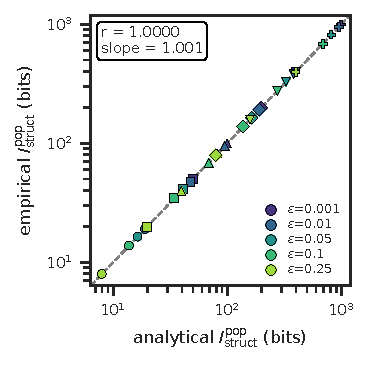
\includegraphics[width=0.31\linewidth]{fig1/fig1_panel_a}}\hfill
\subcaptionbox{\label{fig:apparatus_validation_b}}{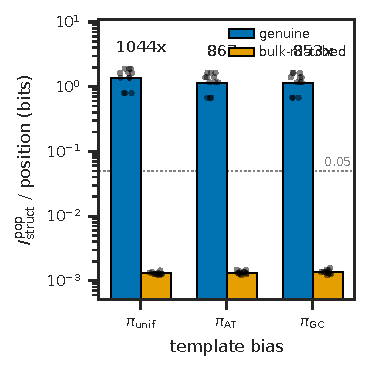
\includegraphics[width=0.31\linewidth]{fig1/fig1_panel_b}}\hfill
\subcaptionbox{\label{fig:apparatus_validation_c}}{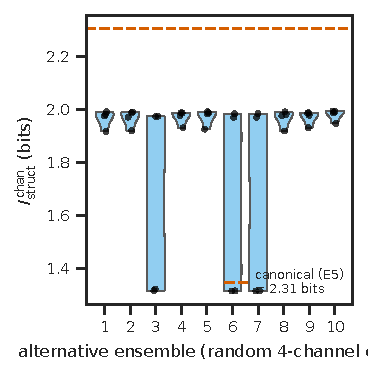
\includegraphics[width=0.31\linewidth]{fig1/fig1_panel_c}}
\caption{\textbf{Apparatus validation and bulk-matched control.} (\textbf{A}) Empirical $\Istructpop$ versus analytical prediction across the $\varepsilon \times L$ sweep, showing close tracking of analytical capacity in noise-free Mode 1 templating (test A1). (\textbf{B}) Separation ratio ${\Istructpop}^{\text{genuine}} / {\Istructpop}^{\text{bulk}}$ across three template-bias conditions, showing $> 20\times$ separation between genuine templating and bulk-matched controls (test A2). (\textbf{C}) Comparison-ensemble robustness: $\Istructchan$ across 11 alternative comparison ensembles (test G3); the qualitative classification of Drt3a as Mode 1 and Drt3b as Mode 3 is preserved across all ensembles, confirming that the apparatus's classificatory verdict is stable under reasonable analyst choices.}
\label{fig:apparatus_validation}
\end{figure*}

\begin{figure*}
\centering
\subcaptionbox{\label{fig:scaling_laws_a}}{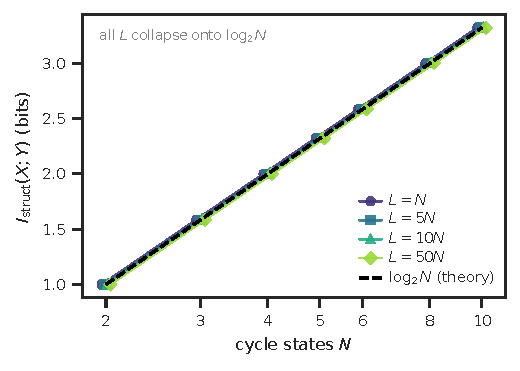
\includegraphics[width=0.46\linewidth]{fig2/fig2_panel_a}}\hfill
\subcaptionbox{\label{fig:scaling_laws_b}}{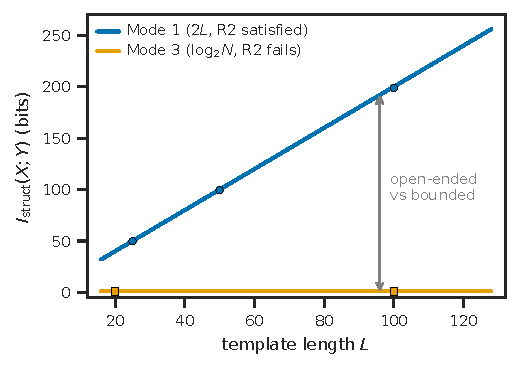
\includegraphics[width=0.46\linewidth]{fig2/fig2_panel_b}}\\[1ex]
\subcaptionbox{\label{fig:scaling_laws_c}}{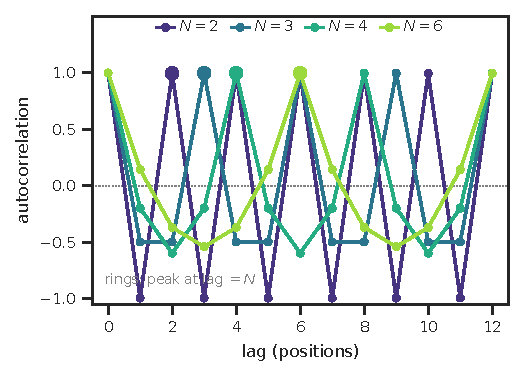
\includegraphics[width=0.46\linewidth]{fig2/fig2_panel_c}}\hfill
\subcaptionbox{\label{fig:scaling_laws_d}}{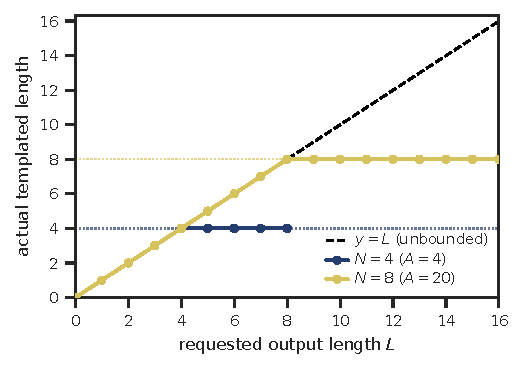
\includegraphics[width=0.46\linewidth]{fig2/fig2_panel_d}}
\caption{\textbf{Mode-specific information-capacity scaling.} (\textbf{A}) Mode 3 information capacity $\Istructpop$ saturates at $\log_2 N$ as cycle states $N$ increase (test B), regardless of template length $L$, confirming that the macro-level capacity bound is set by the cycle's recurrent phase repertoire and not by output length. (\textbf{B}) Mode 1 capacity scales linearly in $L$ (slope $\log_2 |\mathcal{A}| = 2$) while Mode 3 saturates at $\log_2 2 = 1$ bit; the structural difference between (R2)-satisfying and (R2)-failing substrates is visible in this single panel. (\textbf{C}) Mode 3 output autocorrelation peaks at lag $= N$ for $N \in \{2, 3, 4, 6\}$, the canonical signature of cyclic-phase templating. (\textbf{D}) Mode 5 output length is capped at the module count $N$ regardless of requested $L$ (test C), confirming the (R2)-failure-at-module-count diagnosis.}
\label{fig:scaling_laws}
\end{figure*}

\begin{figure*}
\centering
\subcaptionbox{\label{fig:drt3_apparatus_a}}{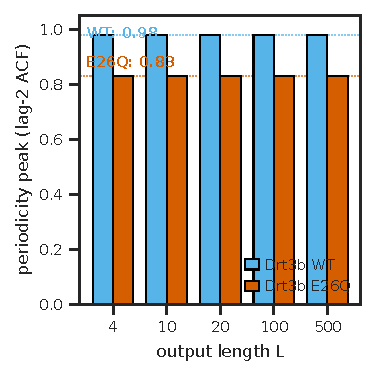
\includegraphics[width=0.31\linewidth]{fig3/fig3_panel_a}}\hfill
\subcaptionbox{\label{fig:drt3_apparatus_b}}{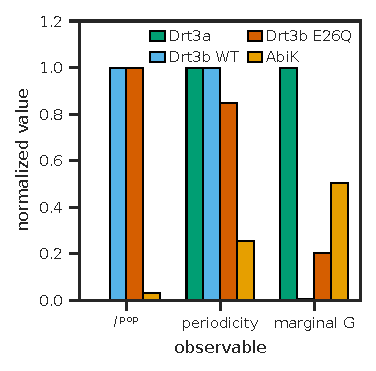
\includegraphics[width=0.31\linewidth]{fig3/fig3_panel_b}}\hfill
\subcaptionbox{\label{fig:drt3_apparatus_c}}{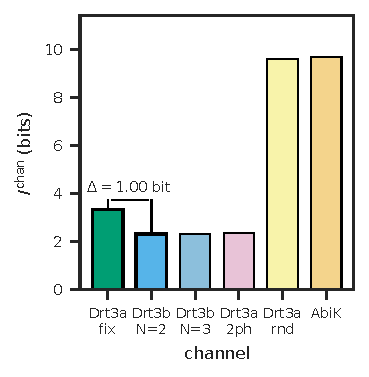
\includegraphics[width=0.31\linewidth]{fig3/fig3_panel_c}}
\caption{\textbf{Apparatus signature on the Drt3 system.} (\textbf{A}) Drt3b WT vs E26Q periodicity peaks (test E2): WT shows $\fphase \approx 0.99$, E26Q shows $\fphase \approx 0.83$, confirming the analytical prediction of half-cycle dG misincorporation in the gate-broken mutant ($0.5 \times 0.20 = 0.10$ marginal G fraction; observed $0.1016$ in Deng et al. 2026 Fig. 4J). (\textbf{B}) Apparatus triple ($\Istructpop$, periodicity peak, marginal G fraction) separating WT Drt3b, E26Q, AbiK, and Drt3a in joint-observable space (test G2); the four systems classify cleanly despite producing nearly identical alternating output for some pairs. (\textbf{C}) Channel-mutual-information separation: against the stated five-channel comparison ensemble, Drt3a-WC channel gives $\Istructchan = 3.33$~bits and Drt3b-N=2 channel gives $\Istructchan = 2.33$~bits, yielding $\Delta\Istructchan = 1.0$~bit between Mode 1 and Mode 3.}
\label{fig:drt3_apparatus}
\end{figure*}

\begin{figure*}
\centering
\subcaptionbox{\label{fig:drt3b_family_a}}{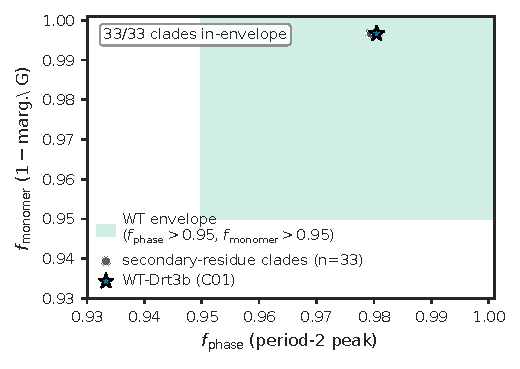
\includegraphics[width=0.46\linewidth]{fig4/fig4_panel_a}}\hfill
\subcaptionbox{\label{fig:drt3b_family_b}}{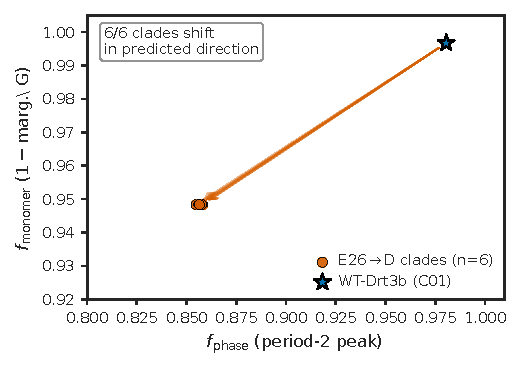
\includegraphics[width=0.46\linewidth]{fig4/fig4_panel_b}}
\caption{\textbf{Drt3b family-level apparatus application across 1{,}232 homologs.} (\textbf{A}) In-envelope behavior of 33 secondary-residue clades (test F): all 33 fall within the WT-Drt3b apparatus envelope, supporting the inference that secondary-residue diversity does not break the cyclic-conformational mode. (\textbf{B}) E26$\to$D selectivity-gate signature in 6 primary-gate clades (C06, C14, C20, C27, C28, C42): marginal G fraction rises from $\sim 0.003$ in WT-like clades to $\sim 0.052$ in the E26$\to$D clades --- a 15.7-fold elevation, consistent with residual hydrogen-bonding flexibility from the shortened Asp side chain. The periodicity peak drops to $\sim 0.857$ as the arithmetic consequence of A-state selectivity loss (analytical $\frac{1}{2}\sum p_A^2 + \frac{1}{2}\sum p_C^2 \approx 0.857$), not as an independent phase failure: cycle architecture is intact (R253 invariant in all 6 clades). All 6 clades show the framework-derived selectivity shift, supporting the classification of E26 as a primary selectivity gate distinct from the architectural gate R253. Apparatus results are computed on Markov channels parameterized from residue assignments at conserved positions, not from raw product sequencing.}
\label{fig:drt3b_family}
\end{figure*}

\begin{figure*}
\centering
\subcaptionbox{\label{fig:inheritance_landscape_a}}{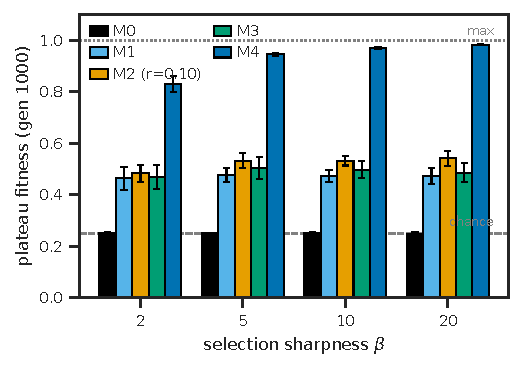
\includegraphics[width=0.46\linewidth]{fig5/fig5_panel_a}}\hfill
\subcaptionbox{\label{fig:inheritance_landscape_b}}{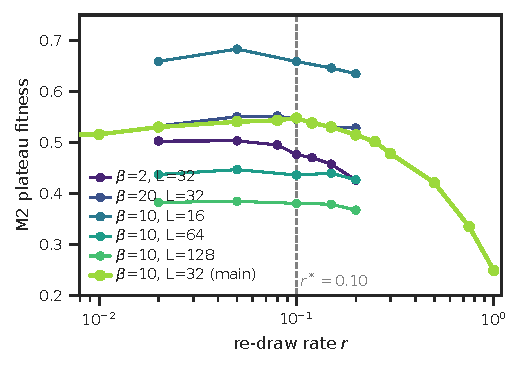
\includegraphics[width=0.46\linewidth]{fig5/fig5_panel_b}}\\[1ex]
\subcaptionbox{\label{fig:inheritance_landscape_c}}{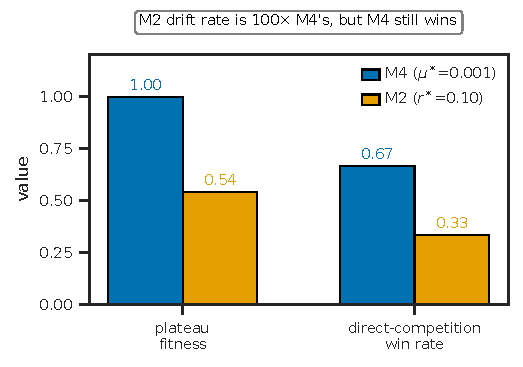
\includegraphics[width=0.46\linewidth]{fig5/fig5_panel_c}}\hfill
\subcaptionbox{\label{fig:inheritance_landscape_d}}{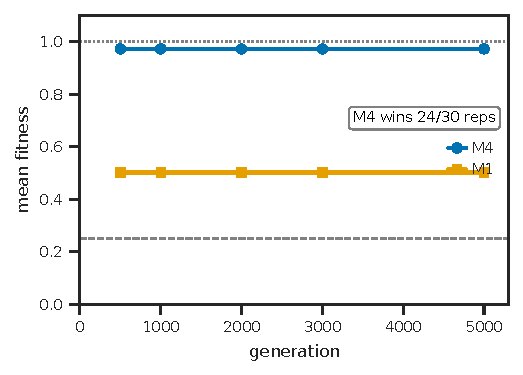
\includegraphics[width=0.46\linewidth]{fig5/fig5_panel_d}}
\caption{\textbf{Population-dynamic plateaus from substrate condition failure.} (\textbf{A}) Mechanism-specific plateau heights $\bar{F}_{1000}$ across selection sharpness $\beta \in \{2, 5, 10, 20\}$ (test H3): M0 (R3,R4 fail) plateaus at chance (0.250); M1, M3 (R4 fails) plateau near initial-population maximum ($\sim 0.47$--$0.50$); M2 at $r=0.10$ (partial R4) plateaus at $\sim 0.53$; M4 (R1--R4 satisfied) reaches $\sim 0.97$. (\textbf{B}) M2 sweet-spot at $r^* \approx 0.10$, regime-invariant within $\pm 0.05$ across $\beta \in \{2, 5, 10, 20\}$ and $L \in \{16, 32, 64, 128\}$ (test H5). (\textbf{C}) M4 vs M2 head-to-head at matched per-offspring drift rate (test H5): M2 introduces 2.40 new positions/offspring at $r^*=0.10$; M4 introduces 0.02 at $\mu^*=0.001$; M4 still wins 67\%/33\% in direct competition, demonstrating that targeted local drift converts to fitness gain more efficiently than wholesale lineage re-draw. (\textbf{D}) Long-horizon (5000 generations) M4 vs M1 trajectories at equal-start initial conditions ($K_{M1} = K_{M4} = 200$): M4 wins 24/30 replicates; M1's plateau is durable but bounded.}
\label{fig:inheritance_landscape}
\end{figure*}

\begin{figure*}
\centering
\subcaptionbox{\label{fig:mode6_cortex_a}}{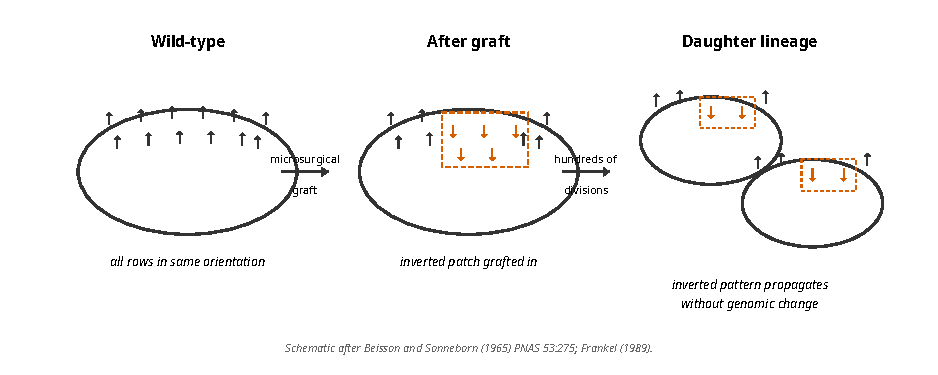
\includegraphics[width=0.30\linewidth]{fig6/fig6_panel_a}}\hfill
\subcaptionbox{\label{fig:mode6_cortex_b}}{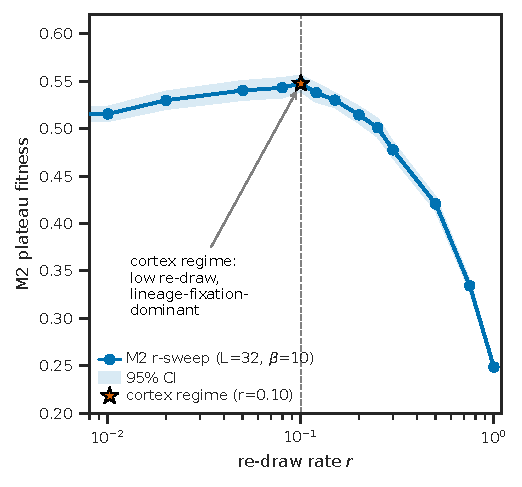
\includegraphics[width=0.31\linewidth]{fig6/fig6_panel_b}}\hfill
\subcaptionbox{\label{fig:mode6_cortex_c}}{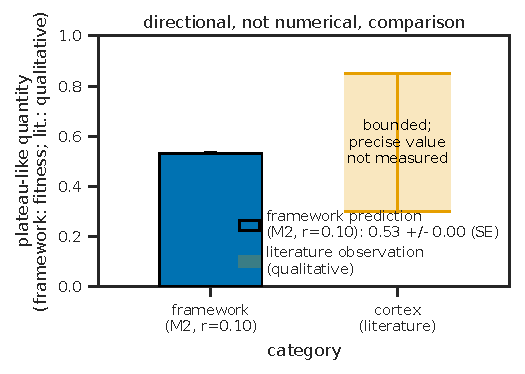
\includegraphics[width=0.31\linewidth]{fig6/fig6_panel_c}}
\caption{\textbf{Mode 6 reframing and ciliate cortex bounded-heredity retrodiction.} (\textbf{A}) Schematic of cortical inheritance after \citet{BeissonSonneborn1965}: a microsurgically grafted patch of inverted ciliary basal-body rows propagates as inverted across hundreds of cell divisions in \emph{Paramecium} without genomic change, demonstrating that the cortex inherits non-genomic structural variation. (\textbf{B}) Operational analog within the M2 mechanism class: at every cell division, cortical units are re-drawn from genome-encoded parts; the existing pattern biases the orientation of newly assembled units. The framework places the cortex in the M2 regime with $r \approx 0.10$ (low re-draw, lineage-fixation-dominant), consistent with the Beisson-Sonneborn observation. (\textbf{C}) Predicted vs observed: the framework predicts bounded but persistent heredity for Mode 6 substrates (M2 plateau at $\sim 0.53$ in our simulation), and the literature reports bounded but persistent cortical inheritance (hundreds of generations of pattern propagation, no qualitatively new cortical structures accumulated over evolutionary timescales). The comparison is directional, not quantitative: the literature's ``bounded heredity'' is a qualitative observation, not a fitness measurement.}
\label{fig:mode6_cortex}
\end{figure*}


\begin{table*}
\caption{\textbf{Substrate recursion principle: four structural conditions plus one scope-defining condition.}}
\label{tab:principle}
\begin{tabular}{p{0.05\linewidth} p{0.18\linewidth} p{0.30\linewidth} p{0.40\linewidth}}
\toprule
Condition & Name & Statement & Failure mode in biological substrates \\
\midrule
R1 & Positive entropy per recognized site & At each addressable position, recognition alphabet $|\Sigma| \ge 2$ with $h_{\mathrm{site}} = \log_2 |\Sigma| > 0$ & Mode 4 (prions, conformer-state): recognition alphabet is small attractor repertoire, $h_{\mathrm{site}}$ bounded at $\log_2 K$ at the macro level \\
R2 & Unbounded independently variable position count & Non-recurrent sites with $\liminf_{L\to\infty} N(L) = \infty$; substrate is not constrained to a finite recurrent phase repertoire (independence in the first-order descriptor-relative sense, not strong joint-statistical independence) & Mode 3 (cyclic): $N(L)$ bounded at cycle length $N$ regardless of product length. Mode 5 (modular): bounded at module count $N$. Mode 4: $N(L) \approx 1$ trivially \\
R3 & Same-operation recursion & Output is structurally readable by the same operation, possibly via reversible involution & Mode 2 (translation): protein product is not ribosome-readable; recursion is parasitic on Mode 1. Mode 5 (NRPS): peptide product is not the assembly line. Mode 6 (cortex): surface does not self-copy autonomously \\
R4 & Heritable local drift in recognized alphabet & Drift lies in the recognition alphabet of (R1); content and templating function are the same physical entity. ``Drift'' rather than ``error'': the kernel produces what its physics produces; the dispersion is a property of the kernel ensemble, not departure from an external target & Crystals (excluded from biology): defect propagation in bounded geometric alphabet, not extensible alphabet. Mode 6: pattern drift independent of genome drift cannot accumulate \\
R5 & Scope: non-teleological intrinsic operation & Operation is intrinsic physicochemistry, not externally specified; no target, loss function, or agent within the operation. Scope-defining: demarcates domain of (R1)--(R4), does not introduce a structural condition & LLM training (non-biological): operations are externally specified by loss function; gradient updates are not substrate-intrinsic recursion. Outside scope rather than structurally failing \\
\bottomrule
\end{tabular}
\end{table*}


\begin{table*}
\caption{\textbf{Six modes of biological templating, classified by substrate recursion principle conditions.}}
\label{tab:modes}
\begin{tabular}{p{0.05\linewidth} p{0.16\linewidth} p{0.18\linewidth} p{0.16\linewidth} p{0.13\linewidth} p{0.20\linewidth}}
\toprule
Mode & Substrate & Conditions failed & Capacity scaling & Copyability & Examples \\
\midrule
1 & 1D linear sequence on separate molecule & None (satisfies R1--R4 within R5 scope) & $L \cdot \log_2 |\mathcal{A}|$ & Auto-catalytic via complementarity (R3 via involution) & DNA replication, Drt3a, retrons, telomerase, DRT9 \\
2 & 1D sequence + separable lookup table & R3 (parasitic recursion via Mode 1) & $\le L \cdot H(\nu)$, code-degeneracy bounded & Via Mode 1 on encoding gene & Ribosomal translation \\
3 & 3D protein with cyclic dynamics, $N$ states & R2 (bounded position count $N$) & $\le \log_2 N$ (saturating) & Not autocatalytically copyable & Drt3b $(N=2)$. DRT7 $(N=1)$ is structural-selectivity boundary, $\log_2 1 = 0$ positional capacity \\
4 & Discrete conformational state & R1 ($h_{\mathrm{site}}$ bounded at $\log_2 K$), R2 ($N \approx 1$) & $O(1)$ length-independent & Propagation, not copy & Prions, amyloids, DRT1 filament \\
5 & Spatial sequence of $N$ modules & R2 (bounded at module count), R3 (parasitic) & $N \cdot \log_2 k$, output bounded by $N$ & Via Mode 1+2 on module gene & NRPS, polyketide synthases \\
6 & 2D pattern (lattice, surface, cortex) & R3 (no autonomous self-copy), R4 (no autonomous heritable drift) & R1, R2 satisfied at surface; bounded by Mode 1 dependency & Limited heredity, parasitic on Mode 1 & Quasicrystal adlayers; ciliate cortex \\
\bottomrule
\end{tabular}
\end{table*}


\begin{table*}
\caption{\textbf{DRT family classification under the framework.}}
\label{tab:drt_family}
\begin{tabular}{p{0.10\linewidth} p{0.18\linewidth} p{0.50\linewidth} p{0.16\linewidth}}
\toprule
System & Mode & Mechanism summary & Reference \\
\midrule
DRT1 & Mode 4 & Filamentous quaternary state with ssDNA effector & \citep{DRT1preprint2026} \\
DRT2 & Mode 1 & Rolling-circle reverse transcription on ncRNA template, \textit{neo} effector & \citep{Wilkinson2024, Tang2024} \\
DRT3a & Mode 1 & Watson-Crick on ACACAC ncRNA region, produces poly(GT) & \citep{Deng2026} \\
DRT3b & Mode 3 ($N=2$) & Cyclic protein-conformational gating, produces poly(AC) & \citep{Deng2026} \\
DRT4 & Out of scope & Random ssDNA, biasing-participant (toxin) & \citep{DRT4paper2025} \\
DRT6 & Out of scope & Random ssDNA, structural homolog of DRT4 & --- \\
DRT7 & Mode 3 boundary ($N=1$) & Single-state arginine-rich pocket, $\log_2 1 = 0$ positional capacity; structural channel selectivity remains, but no positional templating; classified as boundary case rather than full Mode 3 instance & \citep{DRT7preprint2026} \\
DRT9 & Mode 1 & Poly-U ncRNA template, produces poly(dA) homopolymer & \citep{Mou2025} \\
DRT10 & Mode 1 & Translocation-based reuse of short ncRNA template; telomerase ancestor & \citep{DRT10preprint2025} \\
\bottomrule
\end{tabular}
\end{table*}


\begin{table*}
\caption{\textbf{Epistemic status of the Drt3 claims.} Results in this paper fall into four categories. \emph{Observed} = published experimental fact from \citet{Deng2026}. \emph{Derived} = arithmetic or analytical consequence of an observed fact under the framework. \emph{Simulated} = Markov-chain apparatus output on parameters read from the published biochemistry or from structural homology. \emph{Predicted} = framework-derived experimental target not yet measured.}
\label{tab:epistemic_status}
\begin{tabular}{p{0.20\linewidth} p{0.13\linewidth} p{0.55\linewidth}}
\toprule
Claim & Status & Source / basis \\
\midrule
Drt3b produces alternating poly(AC) without nucleic acid template & Observed & \citet{Deng2026} biochemistry \\
E26Q produces 80\%/20\% dA/dG split at A-state & Observed & \citet[Fig.\ 4J]{Deng2026} \\
AbiK same-fold produces random ssDNA & Observed & \citet{Deng2026} \\
1,232-homolog alignment with E26, G248, R253 conservation pattern & Observed & \citet{Deng2026} Data S3 \\
Marginal G fraction $\approx 0.10$ in E26Q (analytical $0.5 \times 0.20$) & Derived & Half-cycle dG misincorporation arithmetic \\
Period-2 self-match $\approx 0.857$ in E26$\to$D clades & Derived & $\frac{1}{2}\sum p_A^2 + \frac{1}{2}\sum p_C^2$ from parameterization \\
Mode 3 capacity ceiling $\log_2 N$ & Derived & Capacity theorem applied to $N$-state cyclic substrate \\
WT Drt3b: $\Istructpop = 1.0$ bits, $\fphase \approx 0.99$, separation ratio $234\times$--$1031\times$ & Simulated & Apparatus on Markov channel parameterized from observed (AC) output \\
E26Q: $\Istructpop = 1.0$ bits, $\fmonomer \approx 0.80$ A-state & Simulated & Apparatus on Markov channel parameterized from observed 80\%/20\% split \\
33/33 secondary-residue clades in-envelope & Simulated & Apparatus on per-clade Markov parameterizations from residue assignments \\
15.7-fold elevated dG in 6 E26$\to$D clades & Simulated & Apparatus on per-clade parameterizations; not measured from raw products \\
Drt3a vs Drt3b separation $\Delta\Istructchan = 1.0$~bit & Simulated & Channel-MI against stated 5-channel ensemble \\
R253A: $\Istructpop \to 0.009$, phase peak $\to 0.43$, cycle collapse & Predicted & SDM experimental target; not yet performed \\
G248A: $\Istructpop$ near WT, marginal G $\to 0.15$, cycle intact & Predicted & SDM experimental target; not yet performed \\
R253A + G248A double mutant: R253A signature dominates & Predicted & SDM experimental target; falsification target for gate-class ordering \\
\bottomrule
\end{tabular}
\end{table*}


\begin{table*}
\caption{\textbf{Universal-gate site-directed-mutagenesis predictions (architectural versus selectivity).} Predictions at $L = 64$, 30 reps, $n_{\mathrm{samples}} = 5000$ per rep. 95\% CIs from beta-binomial.}
\label{tab:sdm_predictions}
\begin{tabular}{p{0.13\linewidth} p{0.13\linewidth} p{0.18\linewidth} p{0.16\linewidth} p{0.16\linewidth} p{0.16\linewidth}}
\toprule
Mutant & Class & $\Istructpop$ (bits) [95\% CI] & Marginal G [95\% CI] & Period-2 peak [95\% CI] & Falsification target \\
\midrule
WT (Drt3b) & --- & 0.9997 [0.9987, 1.0000] & 0.0033 [0.0031, 0.0035] & 0.9802 [0.9794, 0.9808] & --- \\
R253A & Architectural & 0.0090 [0.0065, 0.0120] & 0.1265 [0.1255, 0.1274] & 0.4325 [0.4303, 0.4345] & If observed $\Istructpop > 0.5$ bits, R253-as-architectural-gate claim is wrong \\
R253K & Partial architectural & 0.94 & 0.027 & 0.85 & If WT-like, R253's role is more limited \\
R253H & Partial architectural & 0.85 & 0.068 & 0.70 & Intermediate; checks dose-response \\
G248A & Selectivity & 0.9966 [0.9936, 0.9991] & 0.1516 [0.1505, 0.1528] & 0.7469 [0.7455, 0.7479] & If $\Istructpop < 0.5$ bits, G248 is architectural and gate-class distinction fails \\
G248V & Selectivity & 0.972 & 0.077 & 0.82 & Confirms cycle preserved \\
G248D & Selectivity & 0.971 & 0.102 & 0.79 & Confirms cycle preserved \\
R253A + G248A & Architectural-dominant & 0.0084 [0.0059, 0.0116] & 0.1519 [0.1506, 0.1537] & 0.3872 [0.3855, 0.3892] & If G248A signature dominates, architectural-versus-selectivity ordering is wrong \\
\bottomrule
\end{tabular}
\end{table*}


\begin{table*}
\caption{\textbf{Inheritance-mechanism plateau heights (Test H3, Corollary 2).} Plateau = mean fitness at gen 1000 averaged over 30 replicates. $K = 400$, $L_{\mathrm{TARGET}} = 32$, $\mu_{M4} = 0.01$. Theoretical maximum 1.0; chance baseline 0.250. Mechanism-condition mapping in column 2.}
\label{tab:plateau_heights}
\begin{tabular}{l p{0.30\linewidth} c c c c}
\toprule
Mechanism & Conditions failed & $\beta = 2$ & $\beta = 5$ & $\beta = 10$ & $\beta = 20$ \\
\midrule
M0 (stateless) & R3, R4 & 0.249 & 0.249 & 0.250 & 0.249 \\
M1 (lineage fixation) & R4 (no individual-level drift) & 0.464 & 0.476 & 0.472 & 0.473 \\
M2 ($r = 0.10$) & R4 partial (wholesale re-draw, not local drift) & 0.483 & 0.532 & 0.533 & 0.541 \\
M3 (individual exact copy) & R4 (no drift) & 0.469 & 0.504 & 0.498 & 0.485 \\
M4 (individual + local drift) & None (R1--R4 satisfied within R5 scope) & 0.832 & 0.948 & 0.972 & 0.984 \\
\bottomrule
\end{tabular}
\end{table*}


\section*{Data Availability}

All simulation code, raw simulation outputs, the diagnostic apparatus implementation, the family-level analysis pipeline, and the dispatch markdown files containing the pre-specified analysis plans for each test cohort are deposited in a permanent public repository archived at \zenodoDOI{}. Phylogenetic input files (\texttt{science\_aed1656\_data\_s4--s8}) are derived from the published supplementary material of \citet{Deng2026}. The deposit's git history records the commit ordering: Phase 0 retroactively commits the dispatches with their original filesystem mtimes preserved as commit metadata; Phases 1--5 commit the test scripts, result CSVs, and figure pipeline. The pre-specified predictions are also reproduced verbatim in the docstring headers of the test scripts (e.g.\ \texttt{test\_h\_competition.py}) committed in Phases 2--4.


\bibliographystyle{apsrev4-2}
\bibliography{templating_substrates}

% --- Reference cleanup required in templating_substrates.bib before submission ---
% (1) DRT4paper2025: replace placeholder with verified citation
%     Nat Commun 17, 289 (2026); DOI 10.1038/s41467-025-66997-x.
% (2) DRT10preprint2025: cite as
%     Mou et al., "Antiviral reverse transcriptases reveal the evolutionary
%     ancestry of telomerase," bioRxiv 2025.10.16.682844 (deposited 2025-10-16);
%     DOI 10.1101/2025.10.16.682844.
% (3) DRT1preprint2026 and DRT7preprint2026: verify and replace
%     "{DRT1/DRT7} preprint authors" with named first authors per bioRxiv records.
% (4) BeissonSonneborn1965: ensure citation lands clearly on the
%     "bounded but persistent" cortical-inheritance claim
%     (PNAS 53, 275-282, 1965).

\end{document}
